%%%%%%%%%%%%%%%%%%%%%%%%%%%%%%%%%%%%%%%
%                                     %
%    Header Start                     %
%                                     %
%%%%%%%%%%%%%%%%%%%%%%%%%%%%%%%%%%%%%%%

% Din A 4 page with font size 12
%\documentclass[a4paper, twosides, 12pt]{article}
\documentclass[12pt,a4paper]{article}
\usepackage[english]{babel}
\usepackage[T1]{fontenc}
\usepackage[utf8]{inputenc}

%von niko
%\usepackage[margin=1.5in]{geometry}
%\usepackage{algorithmic}
\usepackage{subcaption}
% \usepackage{float}
% \usepackage{subfloat}
% \usepackage{subfigure}
%\usepackage{lettrine}
%\usepackage[sc,osf]{mathpazo}
\usepackage{booktabs}
% Es wird nicht eingerckt
\parindent=0mm

% arabic numbers for page numbering
\pagenumbering{roman}

% Definition der Ränder
\usepackage[paper=a4paper,left=30mm,right=30mm,top=25mm,bottom=25mm]{geometry}

% for declaring and using colors
\usepackage[table]{xcolor}
% define color values here
\definecolor{myblue}{rgb}{0.94, 0.97, 1.0}
\definecolor{Gray}{gray}{0.8}

% justification of typewriter text
\newcommand*\justify{%
  \fontdimen2\font=0.4em% interword space
  \fontdimen3\font=0.2em% interword stretch
  \fontdimen4\font=0.1em% interword shrink
  \fontdimen7\font=0.1em% extra space
  \hyphenchar\font=`\-% allowing hyphenation
}

% for apacite references
% \usepackage{apacite}
% \bibliographystyle{apacite}

% add references to Table of Contents
\usepackage[nottoc]{tocbibind}

% environment for definitions
\newtheorem{definition}{Definition}

\newtheorem{problem}[definition]{Problem}

% enumerate change
\usepackage{paralist}

% for romanic numbers
\newcommand{\RM}[1]{\MakeUppercase{\romannumeral #1{}}}

% for inserting graphics
\usepackage{graphicx}
% \usepackage{subfigure}
\usepackage{tikz}
\usetikzlibrary{arrows,shapes,positioning,shadows,trees}
\tikzset{
  basic/.style  = {draw, text width=3cm, drop shadow, font=\sffamily, rectangle},
  root/.style   = {basic, rounded corners=2pt, thin, align=center,
                   fill=green!30},
  level 2/.style = {basic, rounded corners=6pt, thin,align=center, fill=green!60,
                   text width=8em},                                                  
  level 3/.style = {basic, thin, align=left, fill=blue!60, text width=6.9em}
}
\usepackage{wrapfig}

\graphicspath{{../results/}}

%\usepackage{pstricks}

% for inserting tables
\usepackage{tabularx, multirow, array, dcolumn}

% for mathematical symbols
\usepackage{amsmath}
\usepackage{amssymb}
\usepackage{latexsym}

% for graphics
\usepackage{tikz}
\usetikzlibrary{arrows,positioning}
\usepackage{color}

%for ipa
\usepackage{tipa}

% pdf LaTeX for linguistic examples
\usepackage{linguex}

%%for OT tables
\usepackage{pifont}    %for pointing hand
\usepackage{arydshln}    %for dashed lines
\usepackage{rotating}    %for angled text

% for inserting pdfs
\usepackage{pdfpages} 

% for inserting trees
\usepackage{qtree}
%\usepackage{ps-trees}

% for line distance
\usepackage{setspace}

% for thick lines
\usepackage{booktabs}

% for footer and header
\usepackage{fancyhdr}

% hyperlink references
\usepackage{hyperref}

%resizing
\usepackage{adjustbox}

% landscape format
\usepackage{lscape}
% for caption formatting
\usepackage{caption}

% for quotation marks
\newcommand{\Gu}{\glqq{}}		% quotation marks top
\newcommand{\Go}{\grqq\xspace} 	% quotation marks bottom
\newcommand{\Ga}{\textquotedblleft{}} % american quotation marks top start
\newcommand{\Ge}{\textquotedblright\xspace} % american quotation marks top end
\newcommand{\Tg}[1]{\textsubscript{#1}}		% lower
\newcommand{\Hg}[1]{\textsuperscript{#1}}	% higher
\newcommand{\leer}{\vspace*{\baselineskip}}% empty line

% reference with \tab, \fig, \sec to tables, graphics, and paragraphs
\usepackage{titleref}
\usepackage{prettyref}
\newrefformat{tab}{siehe Tab. \ref{#1} "\titleref{#1}" auf der Seite \pageref{#1}}% tables
\newrefformat{fig}{siehe Fig. \ref{#1} "\titleref{#1}" auf der Seite \pageref{#1}}% graphics
\newrefformat{sec}{siehe Abschnitt \ref{#1} "\titleref{#1}" auf der Seite \pageref{#1}}% paragraphs
%\pageref{#1}

%changes the numbering of figure and table
\numberwithin{figure}{section}
\numberwithin{table}{section}
\numberwithin{definition}{section}

% heading tweaks
\usepackage{titlesec}
\titleformat{\section}
{\normalfont\Large\bfseries}
{\thesection}
{1em}
{}
\titleformat{\subsection}
{\normalfont\Large\bfseries}
{\thesubsection}
{1em}
{}
\titleformat{\subsubsection}
{\normalfont\Large\bfseries}
{\thesubsubsection}
{1em}
{}

\newcommand{\HRule}{\rule{\linewidth}{0.5mm}}

% global scaling of table size
\usepackage{etoolbox}

\AtBeginEnvironment{tabular}{\scriptsize}
\AtBeginEnvironment{tabularx}{\scriptsize}

% Bibliography
\usepackage[style=authoryear,backend=biber]{biblatex}
\addbibresource{bibliography.bib}

%%%%%%%%%%%%%%%%%%%%%%%%%%%%%
%                           %
%      Document Start       %
%                           %
%%%%%%%%%%%%%%%%%%%%%%%%%%%%%
\begin{document}
\begin{titlepage}
\begin{center}

% Upper part of the page. The '~' is needed because \\
% only works if a paragraph has started.
%\\textsc{includegraphics[width=0.68\textwidth]{bilder/unilogo.png}~\\[1.5cm]
%~\\[1.5cm]
%\vspace{-1.0cm}}

\textsc{\LARGE Master's Thesis}\\[0.8cm]

\textsc{\large in Computational Linguistics}\\[0.5cm]

% Title
\HRule \\[0.4cm]
{  \bfseries \fontsize{22}{37} \selectfont Deconstructing Constructed Languages}\\
\vspace{0.4em}

\HRule \\[1.5cm]



% Author and supervisor
\begin{minipage}{0.4\textwidth}
\begin{flushleft} \large
\emph{Author:}\\
Connor \textsc{Kirberger}
\end{flushleft}
\end{minipage}
\begin{minipage}{0.5\textwidth}
\begin{flushright} \large
%\emph{1st Examiner \& Supervisor:} \\
\emph{Supervisors:} \\
Çağrı \textsc{Çöltekin} \\
Christian \textsc{Bentz}\\
\end{flushright}
\end{minipage}


\vfill



\textsc{\large Seminar f\"ur Sprachwissenschaft\\Eberhard-Karls-Universit\"at T\"ubingen}\\[1.5cm]



% Bottom of the page
{\large December 2023}

\end{center}
\end{titlepage}


%---------------------
% Ende der Titelseite
%---------------------

%----------------------------
% Selbstständigkeitserklrung
%----------------------------

\noindent

Hiermit versichere ich, dass ich die Arbeit selbständig verfasst, keine anderen als die angegebenen Hilfsmittel und Quellen benutzt, alle wörtlich oder sinngemäß aus anderen Werken übernommenen Aussagen als solche gekennzeichnet habe und dass die Arbeit weder vollständig noch in wesentlichen Teilen Gegenstand eines anderen Prüfungsverfahrens gewesen ist und dass die Arbeit weder vollständig noch in wesentlichen Teilen bereits veröffentlicht wurde sowie dass das in Dateiform eingereichte Exemplar mit den eingereichten gebundenen Exemplaren übereinstimmt.\\[4em]
I hereby declare that this paper is the result of my own independent scholarly work.
I have acknowledged all the other authors' ideas and referenced direct quotations
from their work (in the form of books, articles, essays, dissertations, and on the
internet). No material other than that listed has been used.
\\[18mm]
T\"ubingen, \today \hspace{6.0cm} \\%[10mm]\\
\begin{flushright}

\rule{0.4\textwidth}{0.2pt}\\
Firstname Surname
\end{flushright}
\pagestyle{empty}
\newpage

% inserting official anti-plagiarism statement
% \includepdf{antiplagiatserklaerung.pdf}
\newpage
%------------
% Textanfang
%------------

%% Inhaltsverzeichnis
\tableofcontents
\thispagestyle{empty}
%% Anderthalbzeiliger Zeilenabstand ab hier
\onehalfspacing
%\singlespacing

%% Keine Seitenzahl
\pagestyle{empty}

%% Beginn einer neuen Seite
\newpage

%% Abstract
\abstract{

Write the abstract here.
}
\newpage

%% Beginn einer neuen Seite
%\newpage

%%list of figures
\listoffigures
% list of tables
\listoftables


% list of abbreviations
\section*{List of Abbreviations}
\addcontentsline{toc}{section}{List of Abbreviations}

\begin{tabular}{lcl}
\textbf{API} & ~~~ & Application Programming Interface \\
\textbf{NLP} & ~~~ & Natural Language Processing \\
\textbf{PCA} & ~~~ & Principal Component Analysis \\
\textbf{TF-IDF} & ~~~ & Term Frequency - Inverse Document Frequency \\
\textbf{RNN} & ~~~ & Recurrent Neural Network \\
\textbf{LSTM} & ~~~ & Long Short-Term Memory \\
\textbf{SVM} & ~~~ & Support Vector Machine \\
\textbf{XML} & ~~~ & eXtensible Markup Language \\
\textbf{TTR} & ~~~ & Type-Token Ratio \\
\textbf{MATTR} & ~~~ & Moving-Average Type-Token Ratio \\
\textbf{MTLD} & ~~~ & Measurement of Textual Lexical Diversity \\
\textbf{IAL} & ~~~ & International Auxiliary Language \\
\textbf{SVO} & ~~~ & Subject-Verb-Object \\
\textbf{SOV} & ~~~ & Subject-Object-Verb \\
\textbf{IALA} & ~~~ & International Auxiliary Language Association \\
\textbf{LFN} & ~~~ & Lingua Franca Nova \\
\textbf{CSV} & ~~~ & Comma-Separated Values \\
\textbf{MAP} & ~~~ & Maximum a Posteriori \\
\textbf{MSE} & ~~~ & Mean Squared Error \\
\textbf{MDI} & ~~~ & Mean Decrease in Impurity \\
\textbf{MDA} & ~~~ & Mean Decrease in Accuracy \\
\textbf{AUC} & ~~~ & Area Under the Curve \\
\textbf{ROC} & ~~~ & Receiving Operating Characteristic \\
\textbf{PRC} & ~~~ & Precision-Recall Curve \\
\textbf{TP} & ~~~ & True Positive \\
\textbf{TN} & ~~~ & True Negative \\
\textbf{FP} & ~~~ & False Positive \\
\textbf{FN} & ~~~ & False Negative \\
\textbf{SHAP} & ~~~ & SHapley Additive exPlanations \\
\textbf{LIME} & ~~~ & Local Interpretable Model-agnostic Explanations \\


\end{tabular}
\newpage

%\listoftables
%\newpage

%% header with section heading and right-aligned page number
\pagestyle{fancy}
\fancyhf{}
\fancyhead[L]{\textcolor{gray}{\slshape\nouppercase{\rightmark}}}
\fancyhead[R]{\thepage}
\fancyfoot[R]{\textcolor{gray}{Seminar für Sprachwissenschaft Universität Tübingen}}
\renewcommand{\headrulewidth}{0.4pt}

\renewcommand{\headrulewidth}{0.5pt}
\renewcommand{\footrulewidth}{0.5pt}



%--------
% TEXT
%--------
% page numbers start with 1 here.
\setcounter{page}{1}
\pagenumbering{arabic}

\section{Introduction \& Motivation} 
\label{sec:intro}

% Note the choice of "constructed language" in this paper as opposed to other terms, since there is debate, conflation, confusion, and difference in usage at times 

Constructed languages---also called artificial languages, invented languages, planned languages, engineering languages, glossopoeia, or more simply as "conlangs" \parencite{douglas2015book}---are languages that are consciously and purposefully created for some intended use, usually being defined in antithesis to the spontaneous and organic method in which natural languages arise and develop \parencite{sanders2016article}. These variations of the term are often, but not always, used interchangeably, as linguists do not all agree upon a core term due to personal preferences \parencite{Adelman2014article}, and there are sometimes differences in nuance depending on the context in which they appear. This thesis will mainly refer to them as constructed languages for simplicity.

The intended uses for which they are created can range broadly. Some are made specifically for fictional media, often seen in the genres of fantasy or science-fiction, with some more well-known examples being J. R. R. Tolkien's Elvish languages (e.g., Quenya, Sindarin, Nandorin) found in the world of Middle-earth in his writings, Marc Okrand's Klingon language from the Star Trek universe, and David J. Peter's Dothraki language used in George R. R. Martin's A Song of Ice and Fire novels along with their television adaptation, Game of Thrones \parencite{punske2020book}. Others are created to function as international auxiliary languages (IALs)---languages planned for the use of international and cross-cultural communication \parencite{Gobbo2016article}. The most well-known example (based on estimated number of speakers) of these is Esperanto, created in the 19\textsuperscript{th} Century by L. L. Zamenhof. Typically, constructed languages are distinguished and categorized based on these communicative functions. This will be discussed more comprehensively in Chapter \ref{sec:background}. 

% Mention somewhat confusing cases, like "controlled" languages as another example of this blurred line between natural and artificial language or sign languages
% Consciously or subconsciously, conlangs' creators take inspiration and influences from already existing languages, be it natural or even other constructed languages \parencite{Oostendorp2019book}. 

Despite being defined in contrast to one another, however, constructed and natural languages are not necessarily opposite to one another characteristically. Aside from their origins, the boundaries between the two are not always clear when analyzed in greater detail \parencite{goodall2022article}. For example, \textcite{Schubert1989inbook} argues that some languages which are considered "natural" have some degree of artificiality, such as standardized written German and English differing from their spoken forms, and that the reverse is also true of some languages which are considered "artificial" because they draw from aspects of natural languages. As such, he believes human languages exist on a continuum of the two labels, rather than in the binary distinction---a view echoed by other linguists as well \parencite{Novikov2022article}. 

% Mention lack of existing studies specifically comparing/analyzing natural vs constructed languages using machine learning methods
% Expand more on Greenberg and Chomsky principles for linguistic universals, Universal Grammar, etc. and how it relates to this study (Mairal 2006)
% Schubert 1989 argued "no sharp distinction between ethnic and planned languages can be easily found, because any human language can be put in a continuum between naturalness and artificiality"
% Mention interest in deciphering old manuscripts, such as Voynich manuscript or Copiale Cipher, and how such a classification task could be useful in ruling out other possibilities and theories about the text's underlying language (one theory for example is that it's not a natural language)
% [DELETED] The former of the two proposed a framework for identifying the existence and extent of universals in languages based on empirical analysis of their surface structures (i.e. typology)

In many ways, the investigation into the disparity between the these two kinds of languages overlaps with the broader debate regarding what constitutes a language. Central to this debate is the search for linguistic universals---properties shared by all languages \parencite{Mairal2006book}. The concept of universals in language is recognized as one of the most important areas of research in linguistics \parencite{Christiansen2009book} and has served as a foundation for much linguistic theory, especially in more recent history, stemming largely from the influential theories and works of Greenberg \parencite{Greenberg1970book} and Chomsky \parencite{Chomsky1957book,Cook2007book}. 

Analyzing their surface structures can reveal whether or not constructed languages adhere to the same linguistic conventions as their natural counterparts. If machine learning models fail to successfully distinguish between the two, it may reinforce the notion that these universals are present in all languages, regardless of origin. Conversely, the models succeeding may suggest the opposite. In short, the primary motivation behind this thesis is to contribute to this ongoing debate through the application of machine learning, and a desire to learn more about the fascinating genre of constructed languages.

% Furthermore, while research on constructed languages is far from being novel, in the field of computational linguistics it is less common. Thus, my motivation here was to try something relatively new: to formulate this question of binary distinction based on linguistic features into a classification task and use machine learning methods to attempt to answer it.

\subsection{Scope of Study \& Research Question}
\label{ssec:scope}

% Make note of empirical differences between languages such as phonemes, word order, syntax, etc and explain how this study differs/specifies its focus
% [DELETED] As previously noted, the specific boundaries which separate constructed from natural languages are not always clearly or consistently defined---even amongst linguists.

The present work analyzes various linguistic features and seeks to successfully discriminate a language as being either natural or constructed based on these. More specifically, the scope of this study includes both supervised binary classification and unsupervised anomaly detection, with the models being trained on a set of selected features rather than raw text data. 

Because of the wide-ranging nature of conducting such a broad analysis, there are of course many features left unconsidered or excluded, intentionally or otherwise. With this in mind and following the precedent set by other related research on this topic, the main focus for linguistic features relate to entropy, morphological complexity, and overall lexical diversity.

The following is a breakdown of the structure of this thesis from here onward: the next chapter provides relevant background information, including an overview on constructed languages and a comprehensive review of related literature that examines the prior theoretical groundwork laid for exploring linguistic similarities and differences between constructed and natural languages; Chapter \ref{sec:methodology} covers in detail the methodology taken in this research, from an explanation of the data used to the various experiments performed; Chapter \ref{sec:results} presents the results of the study and discussion of these follows in Chapter \ref{sec:discussion}; lastly, Chapter \ref{sec:conclusion} consists of a conclusion as well as elaboration for possible future work.

\newpage
\section{Background}
\label{sec:background}

The vast landscape of linguistic research comprises a myriad of literature delving into the intricacies of languages, both natural and constructed. As this thesis is concerned with constructed languages in particular and possible distinctive properties they may have, this section begins with a brief overview of their history and development, which provides some relevant context. Following this is an overview of some related literature, which is relevant to understanding the motivation behind the various computational approaches I employ in my experiments. 

\subsection{History of Constructed Languages}
\label{ssec:historyofconlangs}

% How much discussion here should overlap or be mutually exlcusive from the later section of me describing the data and languages used. Where would some of this information best fit? Or should I reorganize the sections? I feel I need to give a background on the history of constructed languages, since it's relevant here anyways and it includes a lot of information about the languages I'm using in particular. But then later during the data section of the methodology, I at one point thought to give brief descriptions of them there and introduce them. How should I organize and do this?
% Discuss the history of constructed languages, beginning with so-called philosophical languages of the 17th century (Goodall 2022)
% Discuss different theories of classifying/defining natural from constructed languages
% Other criterion for distinguishing types of constructed languages: a priori vs a posteriori dichotomy (Novikov 2022) and exoteric vs. esoteric dichotomy (Gobbo 2011) 
% Related quote: "The question is at what point we can call a constructed object a language. A useful taxonomy has been proposed by Blanke (1989), who envisaged a three-way distinction of ‘projects’, ‘semi-languages’ and ‘languages’, where ‘projects’ are basically objects which never grew out of the initial grammars and lexicons written by their constructors. They can grow into ‘semi-languages’ and eventually ‘languages’ if they start satisfying a whole list of criteria such as being used in written communication in books and journals, or having specialized vocabulary about a number of topics, etc. where languages are distinguished from semi-languages by having native speakers. According to Blanke, Esperanto is the only full ‘language’ in the set of constructed objects; as Blanke was a leading figure in the Esperanto movement" - Oostendorp
% Mention critique of eurocentrism surrounding constructed languages (the influences/inspirations they derive from), mentioned in Novikov 2022 page 9
% Related to above, Gobbo 2016 section 3 discusses international auxiliary languages including the sourcing of esperanto from western european languages (same for interlingua)
% Type of planned/constructed language makes a difference; Gobbo 2016 says "The ultimate goal of the planned language is important. Secret languages present different characteristics compared to IALs like Esperanto or Volapük: in order to preserve their secrecy, they often show morphological irregularities, in order not to be decrypted by the casual reader. As a consequence, secret languages do not necessarily show grammar reduction and morphological simplicity."
% Gobbo 2016 (page 39) mentions surface level differences in linguistic complexity between constructed and natural languages: " For ‘grammar reduction’, authors generally refer to the fact that planned languages show evident patterns of regularity in word formation, compared to natural languages, with few allomorphs, if any. For example, in English the plural of nouns is realized with various allomorphs (cat/cat-s, fox/fox-es, etc) while in Volapük, the first planned language with a community of supporters (see Section 4 below), there is only one form (vol/vol-s, pük/pük-s, ‘world/worlds’, ‘language/languages’), i.e. there is no allomorphy. Under the assumption that a language with less allomorphy is less complex, we conclude that Volapük is morphologically less complex than English."
% Important distinction when discussing planned languages: Gobbo 2016 writes "An important problem in such a comparison lies in the specificity of planned languages from a sociolinguistic point of view. Language architects can be traced in the development of many natural languages, such as Pompeu Fabra in the case of Modern Catalan (Costa Carreras, 2009), or Alessandro Manzoni in the case of Italian (Gensini, 1993). Pompeu Fabra and Alessandro Manzoni reshaped existing languages, which are alive thanks to a speech community that is actively involved in maintaining and promoting them. In other words, without a speech community, no language planning is possible. This process of reshaping is called ‘Ausbauization’ by Tosco (2011), from the classic term ‘Ausbau’ introduced by Kloss (1967)." In other words, the phrase 'language planning' can refer to actions taken for what are considered natural languages, too. Thus it is important to specify and distinguish this 
% On the origins of differentiating between purposes of constructed languages: Gobbo 2016 says "Alessandro Bausani (1974, 1970) was the first to notice that planned languages can be invented for different purposes."
% Don't forget to discuss Lingua Franca Nova too
% Okrent (2009) - "The history of invented languages is, for the most part, a history of failure."
% Mention sign languages, including Nicaraguan sign language
% italics for a prior and a posteriori?
% Contemporary conlangs are usually developed for one of three purposes: (i) to be an inter- national auxiliary language, known as an auxlang; (ii) to be a language used for an artistic endeavour, known as an artlang; or (iii) as a means of exploring certain philosophical concepts through constructing a language that embeds them, sometimes known as an engelang [2]. Constructed languages have also been categorized in terms of their method of creation. An a posteriori language is one that has been developed using aspects of other naturally occurring languages, while an a priori language is one that is created without intentional use of specific languages (Schreyer 2021)
% "planned languages are by definition based on the priority of writing over speech: they violate the priority of the spoken language over writing, one of the fundamental properties of natural languages, according to theoretical linguistics (Lyons, 1981, Section 4.2.1).2" (Gobbo 2017)
% "Despite the opportunities offered by the new technology, some of the online practices have been deemed questionable by the more scrupulous members of the conlang community: Google Translate offers Esperanto as one of its non-experimental languages, Wikipedia is available in eight different constructed languages (Esperanto, Volapuk, Ido, Interlingua, Kotava, Occidental, Lingua FrancaNova, Novial, Lojban) with Volapuk accounting for the largest number of articles (over 117,000, which places it 17th in the global rating, above the natural languages with millions of speakers), yet the overwhelming majority of them are the examples of low-quality machine translation." (Novikov 2022)

\textcite{okrent2009book} states, "The history of invented languages is, for the most part, a history of failure." She may be justified in saying this, depending on one's definition of failure in this context. From past to present, the total number of constructed languages may be as high as a thousand \parencite{Libert2016inbook,Schubert1989inbook,Schubert2001book}, with hundreds proposed for the purpose of being IALs in Europe alone \parencite{Schubert2001book}. Yet of these, only Esperanto is commonly considered to be successful in achieving its creator's intended goal of world-wide use as an auxiliary language (or rather that it is by far the most successful), with very few others even coming close, having a conservative estimation of two million speakers \parencite{okrent2009book}.

While the construction of languages is possibly as old as human history, they typically were not written down and were limited to in-group communication \parencite{Gobbo2016article}. The first documented endeavors came out of religious contexts and were likely used as secret languages, intentionally obscured and incomprehensible to lay people. In the 12\textsuperscript{th} century, abbess Hildegard of Bingen described and recorded a lexicon for Lingua Ignota, a Latin name meaning "unknown language". While extensive documentation of it (i.e., a grammar) was never found, it possessed a semiotic system based on Latin, German, and Greek. Later in the 14\textsuperscript{th} century, a group of Sufi mystics created Balaibalan, a language written in the Ottoman Turkish alphabet and which incorporated features of Persian, Turkish, and Arabic languages \parencite{Novikov2022article}.

Interest in creating such languages picked up in the 17\textsuperscript{th} century with the rise of so-called philosophical languages. In contrast to the last two, these languages were made to be more precise, less ambiguous, and better allow for philosophical reasoning (compared to natural language), such as by organizing world knowledge into hierarchies \parencite{goodall2022article}. Notable figures involved in making these include Francis Lodwick, Gottfried Leibniz, and John Wilkins, the latter of whose being arguably the most well-known and influential. Wilkins created a system of semantic categorization, cataloging all concepts in the universe \parencite{okrent2009book}, and then published his proposed language \parencite{Wilkins1968book}. An example of this hierarchal categorization can be seen in Figure \ref{fig:wilsonslanguageexample}.

% Include figure of Wilson's work or is it unnecessary? 

\begin{figure}
  \centering
        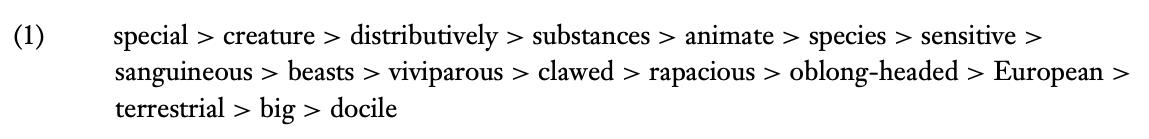
\includegraphics[width=\textwidth]{./Other/WilsonsLanguageExample.png}
        \caption{Wilson's expression of "dog" in his philosophical language \parencite{goodall2022article}.}
        \label{fig:wilsonslanguageexample}
\end{figure}

% It is from this category that the constructed languages used in the present study come from.
% Speak more about details of these IALs here? Or in the data section?

In the 19\textsuperscript{th} and 20\textsuperscript{th} centuries the focus for language construction, especially in Europe, shifted to that of making international auxiliary languages (IALs) intended to better enable communication across language barriers, i.e., people who do not share a similar language \parencite{goodall2022article}. Notably, this means they were generally (though not always) designed to resemble natural language, with choice exceptions being the simplification of certain linguistic features. The surge in need for IALs correlated with the increase in prevalence and accessibility regarding international travel and communication at the time. Such languages were also described as "neutral" \parencite{Large1985book}, in the sense that individual advantages amongst speakers and learners would, theoretically, not exist due to IALs being second languages to everyone \parencite{Gobbo2016article}. That being said, many of the most prominent examples (e.g., Volapük, Interlingua, Esperanto, Ido) are derived from the Indo-European language family \parencite{Novikov2022article,goodall2022article}, so such a description might not be apt. Overall, IALs can be viewed as an intended rival to natural languages, which is one reason why all of the constructed languages analyzed in the present work are IALs. A more detailed explanation of each is provided in Section \ref{ssec:data}

% Discuss all of the IALs here? Or in the Data section instead? Or is it unnecessary to discuss them in such detail anyways?
% [DELETED] clubs were soon founded and spread around Europe and then to the United States and China, too \parencite{okrent2009book}. At its peak nearly a decade later, there were over two hundred societies and clubs, three hundred learning manuals \parencite{Gobbo2016article}, and twenty-five routinely published Volapük journals \parencite{okrent2009book}.
% (Gobbo 2008) for discussing Ido

% [DELETED] As the constructed languages examined and used in the dataset of the present work are all IALs, it would be beneficial to introduce them in more detail here. Volapük was made in 1879 by Catholic German priest Johann Martin Schleyer, who believed it was given to him by God. Argued to be the first successful constructed language due to amassing so many supporters \parencite{Gobbo2016article}, it soon died out in favor of Esperanto, which Ludwik Lejzer Zamenhof published in 1887.

% Mention other kinds of constructed languages, i.e. experimental or artistic ones like Solresol, Laadan, Lojban? (Adelman 2014)

Lastly, there exist constructed languages that have been made for experimental, artistic, literary, or fictional purposes. In contrast to IALs, these languages are not made with the intention of replacing existing languages for everyday communication. Instead, their creators want to push the boundaries of language, test scientific hypotheses like linguistic relativity, or create a world, as is the case for the fictional examples provided in Chapter \ref{sec:intro}. Some other examples in this category include Solresol, a language that uses musical notes; Láadan, a language designed to be inherently feminist (i.e. more capable of expressing the female experience); and Loglan, a self-described "logical" language whose morphology and syntax are based on predicate logic \parencite{Adelman2014article}. Though it would be inaccurate to describe such languages as being only a recent invention, popularity in their conceptualization largely grew in the later part of the 20\textsuperscript{th} century.

While all share the defining characteristic of having been purposefully created, the linguistic features of constructed languages (e.g., phonetic, morphological, syntactical, lexical, orthographic) can vary immensely depending on factors such as their intended purpose for use or the other languages they draw from. An example of this was observed by \textcite{Gobbo2016article} in secret languages, specifically their tendency to have more complicated features, such as morphological irregularities, "in order to preserve their secrecy." Contrast to this are IALs, which have the opposite tendency for the sake of ease of communication and second-language acquisition, reflected in commonly assigned features such as SVO word orders, head-initial relative clauses, fronted \textit{wh-}phrases, and morphological regularity \parencite{goodall2022article,Gobbo2016article}. Section \ref{ssec:priorstudies} further examines research focused on linguistic features of these languages. 

% Include chart "taxonomy of planned languages" from Gobbo 2016 (fig 2). IMPORTANT QUESTION!!!!!! IS IT OKAY TO BORROW DIRECTLY LIKE THIS AS LONG AS I CITE IT?

\begin{figure}[!h]
  \centering
        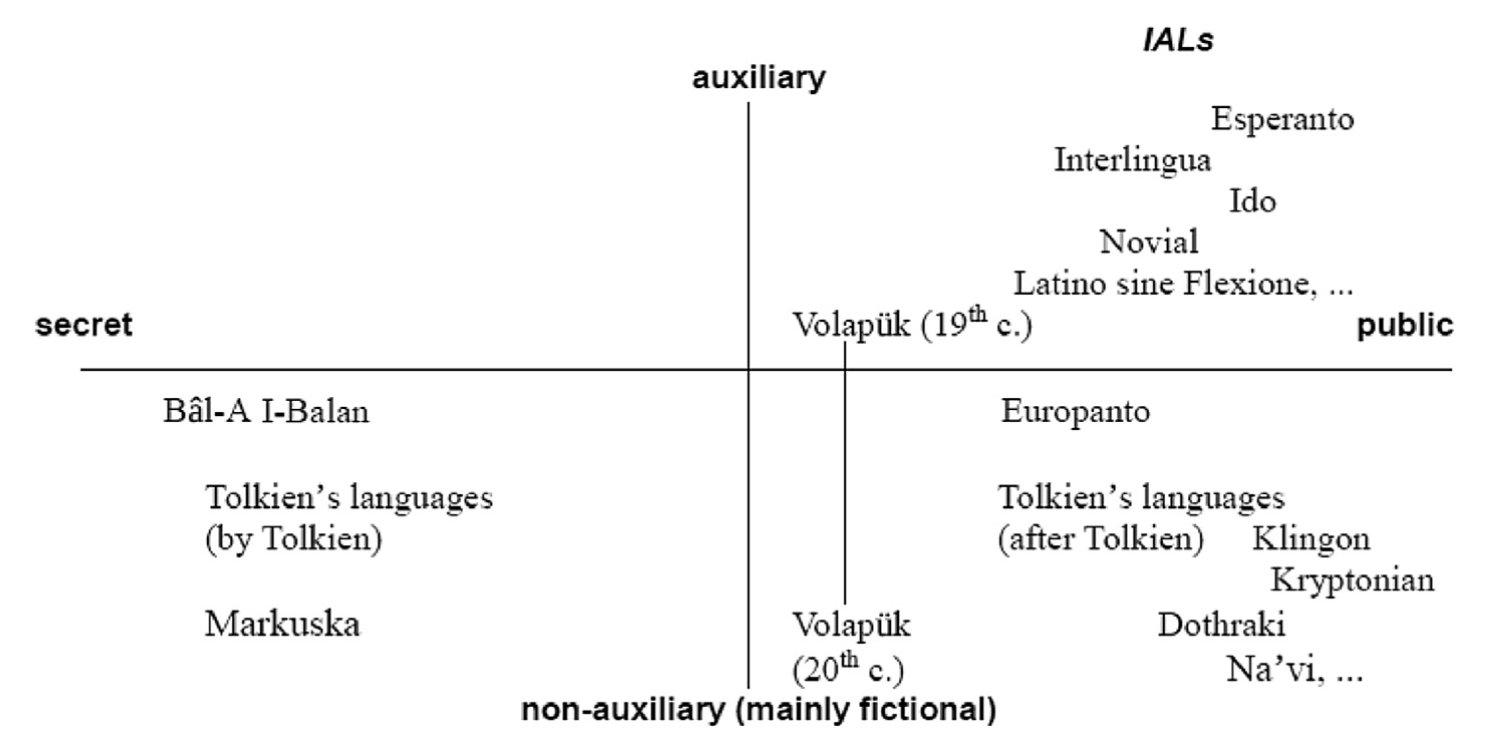
\includegraphics[width=\textwidth]{./Other/TaxonomyOfPlannedLanguages.png}
        \caption{A taxonomy of constructed languages \parencite{Gobbo2016article}.}
        \label{fig:taxonomyplannedlanguages}
\end{figure}

In addition to this classification based on their intended communicative functions, i.e. as philosophical or international auxiliary languages, there are also taxonomies based on other criterion. For example, another frequently used distinction is that of \textit{a priori} and \textit{a posteriori} \parencite{Schreyer2021article,Gobbo2008article,Schubert1989inbook,Schubert2001book,Novikov2022article,Adelman2014article,Tonkin2015article}. Languages described as being \textit{a priori} are structurally entirely new \parencite{Tonkin2015article} and not based on existing languages, whereas so-called \textit{a posteriori} languages are the opposite, drawing from aspects of specific natural languages \parencite{Schreyer2021article}. \textcite{Gobbo2008article} also proposed the dichotomy of \textit{exoteric} (secret) and \textit{esoteric} (public) languages, derived from \textcite{Bausani1974book}. Similar to critiques regarding the distinction between constructed and natural, such dichotomies for categorizing constructed languages are also argued by some linguists to be more accurately described as scales instead, with many languages falling somewhere in the middle \parencite{Novikov2022article}. A final noteworthy classification scheme often cited by other linguists comes from \textcite{Blanke1989book} in the form of three classes: project, semi-planned, and planned. In short, these correspond to a set of steps that a constructed language must go through before it can be considered a "real" language \parencite{Schubert2001book}. 

A two-dimensional taxonomy for constructed languages containing several notables examples is shown in Figure \ref{fig:taxonomyplannedlanguages} \parencite{Gobbo2016article}.

\subsection{Prior Studies}
\label{ssec:priorstudies}

% Prior studies comparing natural and constructed languages by linguistic features, prior studies on classification tasks for constructed languages

% Examining the Inductive Bias of Neural Language Models with Artificial Languages (White 2021)
% Are planned languages less complex than natural languages? (Gobbo 2016) 
% Constructed languages are processed by the same brain mechanisms as natural languages (Malik 2023)
% Constructive Linguistics for Computational Phraseology: the Esperanto Case (Gobbo 2019)
% On Pragmemes in Artificial Languages (Libert 2016)
% Authorship attribution, constructed languages, and the psycholinguistics of individual variation (Juola 2017)
% Sign language : a systematic review on classification and recognition (Sasidharan 2024)
% Morfessor-enriched features and multilingual training for canonical morphological segmentation (Rouhe 2022)
% A Morphological Lexicon of Esperanto with Morpheme Frequencies (Bick)
% How European is Esperanto? (Parkvall 2010)
% Complexity measurement of natural and artificial languages (Febres 2014)
% Native Esperanto as a test case for natural language (Lindstedt)
% Natural and Artificial International Languages: a Typosogist's Assessment (Comrie 1996)
% Evaluating the Irregularity of Natural Languages (Gomez 2017)
% From Esperanto to Volapük: A Graph-Based Approach to Assessing the Complexity of Constructed Languages (Sokolova)
% The word entropy of natural languages (Bentz 2016)
% Entropy of natural languages: Theory and experiment (Levitin 1994)
% Questions in Natural and Artificial Languages (Moskovsky)
% Morphology Matters: A Multilingual Language Modeling Analysis (Park 2021)
% Can Type-Token Ratio be Used to Show Morphological Complexity of Languages? (Kettunen 2014)
% Comparing comparatives in artificial languages
% What do complexity measures measure? Correlating and validating corpus-based measures of morphological complexity (Coltekin 2022)
% The effects of type and token frequency on word length: a cross-linguistic study (Berg 2022)
% Token-based typology and word order entropy: A study based on Universal Dependencies (Levshina 2019)
% Crosslinguistic Corpus Studies in Linguistic Typology (Schnell 2022)
% Data-driven Model Generalizability in Crosslinguistic Low-resource Morphological Segmentation (Liu 2022)
% The development of morphological complexity: A cross-linguistic study of L2 French and English (De Clercq 2016)
% Morpheme-Based Neural Machine Translation Models for Low-Resource Fusion Languages (Gezmu 2023)
% Bentz's papers
% Using the Relative Entropy of Linguistic Complexity to Assess L2 Language Proficiency Development (Sun 2021)
% Multiple studies on artificial language acquisition
% Prior studies on entropies of languages
% Prior cross-linguistic studies examining linguistic features like TTR of constructed/natural languages
% (Gobbo 2016) "The literature on planned languages is abundant and diverse, written in many languages and quite often outside of the usual peer-review system (Blanke, 2003), but in comparison to natural languages there are only few specific studies addressing the complexity of planned languages from the point of view of learnability. For instance, Jansen (2012) addresses the problems of learning the reflexive pronouns in Esperanto. In his review of the doctoral dissertation of Heil (1999), who compares the grammar reduction in French-based creoles and planned languages, Haitao (2001) rightly points out that more comparative work in this field is needed, and on a more solid basis."
% Performance of Robust Support Vector Machine Classification Model on Balanced, Imbalanced, and Outliers Datasets (Sembiring 2024)

% Evaluating the irregularity of natural languages (Gomez 2017) approximates entropy of written texts and finds differences between language families, also compares their results to Esperanto
% Discuss research and the justification for using  one-class svm, decision tree, and randomforest for outlier detection/binary classification

In contrast to the abundance in literature and cross-linguistic analyses done on natural languages, similar research which also includes constructed languages is relatively sparse. In particular, while there is research that analyzes specific instances of linguistic differences between certain natural and constructed languages, large-scale cross-linguistic studies which utilize computational methods to classify the two based on linguistic features are practically nonexistent. Consequently, the present study is a somewhat novel approach. However, there is precedent for this research and the specific features examined, as well as computational approaches used, which this section will describe.

As noted in the previous section, the creation of IALs often involved the intentional simplification of particular linguistic features to facilitate language acquisition, for instance having more regularity in their morphological systems. Intuitively, then, one would assume this translates to measurable differences in various aspects of linguistic complexity when compared to natural languages, which often have irregularities as a result of their development and evolution. When comparing Volapük and English, \textcite{Gobbo2016article} concluded that

Much of the literature on constructed languages focuses on Esperanto specifically.

\subsubsection{Studies in Morphological Complexity}
\label{morphologicalcomplexitystudies}

\subsubsection{Studies in Entropy}
\label{entropystudies}

Another feature examined is entropy. Originating from information science, entropy was introduced by \textcite{Shannon1948book} as a measurement of uncertainty or surprisal for an event, with high surprisal being inversely proportionate to the amount of information conveyed by the event's occurrence. In NLP, 

Many studies into the entropy of natural languages have been conducted, but less so regarding constructed languages. \textcite{Smaha2015book} investigated and compared two constructed languages (Lojban and Klingon) with several natural languages and other artificial languages (e.g., Fortran, a programming language) using calculations of block entropy (Shannon's entropy generalized to n-grams). While broad observation of the results found both Klingon and Lojban to have comparable entropies to the natural languages, closer analysis revealed them to actually be closer to Fortran instead. 

\subsubsection{Computational Approaches}
\label{ssec:computationalapproaches}

\textcite{Oktafiani2024article} 

\newpage
\section{Methodology}
\label{sec:methodology}

In this section, I introduce the dataset for this thesis and discuss the steps taken for preprocessing it, followed by discussing in detail the features examined along with the different methods involved in extracting them from the data, and finally the classifiers employed on the feature set. A brief description of the various APIs and libraries used is also included in \ref{ssec:librariesandapis}. 

Since this study involves many different experiments and elements being performed and analyzed, I will begin by explaining an overview of what all was done. The number of possible features and measurements of linguistic complexity which could be analyzed in such a study is extensive to say the least; however, the scope of this thesis focuses mainly on empirical measurements relating to lexical diversity, morphological complexity, and entropy, along with some other measurements which are commonplace to calculating linguistic complexity, and thus seemed appropriate to also include. More specifically, the features investigated are average word length, average sentence length, type-token ratio (TTR) of morphemes, average number of segmentations in a word, average number of forms per lemma, lexical TTR, moving-average type-token ratio (MATTR), measurement of textual lexical diversity (MTLD), lexical entropy, reverse lexical entropy, text entropy, and character and word distribution entropies. Once the values of these were calculated for each language, the task became that of supervised binary classification and unsupervised anomaly detection with five machine learning models: a one-class support vector machine (SVM), local outlier factor, random forest, isolation forest, and decision tree. Principal Component Analysis (PCA) was also performed on the feature set. Lastly, the methods for evaluating the performances of these models and interpreting them based on feature importance are discussed.

\subsection{Data}
\label{ssec:data}

% Note the reasoning behind the choice of having a dataset with diverse typological features

In total, twenty-four languages are analyzed in this study. Six of these are constructed languages: Esperanto, Ido, Interlingua, Lingua Franca Nova, Volapük, and Kotava. The remaining eighteen are natural: German, English, Spanish, Polish, Vietnamese, Indonesian, Turkish, Tagalog, Hungarian, French, Finnish, Italian, Dutch, Occitan, Danish, Swedish, Afrikaans, and Icelandic. The rationale behind this particular selection of languages will be discussed in further detail throughout this section, but the primary focus was on having diverse typological linguistic features represented in the data.

For consistency, only languages which are written using the Latin alphabet (including the use of diacritics) were chosen. This is mainly because the constructed languages in the dataset all use Latin alphabets, so the selection of natural languages followed the same criteria. Moreover, it allows for more uniform cross-linguistic analysis of features which may be sensitive (e.g. in the case of character entropy) to writing systems.

% Plot the languages + their language families to have some kind of visual comparison (table also works, include some data points for comparing each language i.e. number of speakers, word order (what do I do when it isn't clear due to having a more free word order, like for Esperanto, Finnish, etc?))
% Explain why I had to build my own corpus rather than using one that already exists. What limits are present as a result of having to build my own? 
% Discuss their language families, writing scripts (why not Japanese or Chinese?), and why those 6 constructed languages specifically
% Explain which natural language families the conlangs are based on, and surface level distinctions they may have
% von Oostendorp's Constructed Language and Linguistic Theory cites information about Ido (and Interlingua) around pages 7-8, how it is different from Esperanto
% Write more in-depth about Ido, Esperanto, Interlingua, Volapük, and Lingua Franca Nova. Who created them, how many estimated speakers, their purpose for being created, etc. etc.
% Write differences between Ido and Esperanto, using specific examples (for ex, from Goodall 2022), same for Interlingua. For example, a chart comparing words/grammar in all the languages, like on page 6.
% Mention how for some calculations done in this work, such as entropy, domain and corpus size are important and can cause results to vary
% Comrie 1996 also breaks down Esperanto with examples
% Lindsedt 2006 writes about considering Esperanto as a natural language and breaks down properties of it as well. Gobbo 2011 (section 4) breaks down further the specific languages Esperanto comes from
% Write about the Eurocentricism of the constructed languages used here (their inspirations/influences) and how that may affect the results
% Mention the drawbacks of relying on Wikipedia data, such as difference in authors, etc
% Why didn't include lojban? or Novial? (Available data for it is way smaller)
% Discuss number of symbols (i.e. letters in the alphabet) for each language too

\subsubsection{Constructed Languages in the Dataset}
\label{ssec:constructedlanguagesinthedataset}

% Refer to https://docs.verbix.com/Conlangs/ for more info of these

All of the constructed languages in the dataset are IALs, with most of them resembling natural (particularly various European) languages. I will briefly introduce each of them in this section, explaining where they come from, some notable typological features they have, and how they compare to both one another other and their natural counterparts.

Esperanto, the most widely-spoken constructed language and considered by many to be the most successful \parencite{Gobbo2008article}, was created in 1887 by Polish ophthalmologist L. L. Zamenhof. Zamenhof’s goal was to create a neutral, easy-to-learn language that would facilitate international communication. Esperanto is a highly regular language, with consistent grammar and a simplified, phonetic spelling system. It draws its lexical roots and syntax primarily from Romance, Germanic, and Slavic languages \parencite{Gobbo2008article,Gobbo2011article}, making it recognizable and familiar to speakers of many European languages, while also intentionally being made to have a comparatively simpler grammar that avoids some complexities found in natural languages, such as irregular verbs or noun cases. Its morphological system is considered to be one of its more interesting aspects due to its classification being a source of debate amongst linguists \parencite{Reagan2019book}. It also has a strong global community with speakers around the world, an array of written literature, and even a number of native speakers who learn it from birth---a distinguishing trait which sets it apart from other constructed languages \parencite{goodall2022article}. As a result of its success, Esperanto also serves as a direct influence for many other constructed languages that have come after it, one being Ido. 

% [DELETED] Like most of the remaining constructed languages to be discussed in this section---with the exception of Volapük---Ido has small but a dedicated community of speakers and enthusiasts.

Ido is a reform of Esperanto that was proposed in 1907 by a group of linguists led by Louis Couturat, a French philosopher and mathematician, and in fact is an Esperanto word meaning "offspring" \parencite{Schubert2001book}. Its creators sought to address what they saw as imperfections in Esperanto, particularly those related to orthography, morphology, and lexicography \parencite{Novikov2022article}. For instance, Ido avoids the use of the accusative case and reforms some Esperanto words to make them more universally recognizable. Overall, though, Ido still retains much of Esperanto’s vocabulary and basic structure, and the two are mutually intelligible to a large extend \parencite{goodall2022article,Schubert2001book}.

Interlingua was developed by the International Auxiliary Language Association (IALA) with the assistance of linguist Alexander Gode, officially being published in 1951. A central idea to its creation was that it would be most recognizable to the greatest number of people without requiring prior study \parencite{goodall2022article}, particularly in regards to its lexicon. The IALA's stated goal was to not so much create a new international language, but rather present a standardized international vocabulary \parencite{Large1985book} ("international" here basically referring to Western Europe). It is largely derived from and resembles Romance languages (with lesser influence from Greek and Germanic languages) \parencite{Schubert2001book}. In fact, this intentional resemblance extends even to morphological irregularities such as allomorphy, with other irregularities also being introduced to the language to make it appear more natural \parencite{goodall2022article,Schubert1993article}, a contrast to other IALs like Esperanto \parencite{Gobbo2016article}.

Volapük was created in 1879 by Johann Martin Schleyer, a German Catholic priest who believed the language had been given to him by God. It features highly agglutinative structure and regular, yet complex, morphology \parencite{Reagan2019book}. While being derived mainly from English, German, and Latin, roots in Volapük differ significantly to the point of being unrecognizable to speakers of these languages \parencite{goodall2022article}. Despite being argued to be the first successful constructed language due to its rise in popularity, having amassed a large number of supporters worldwide along with the formation of clubs and societies \parencite{Gobbo2016article}, various issues regarding its complexity led to a rapid decline and eventual fall from usage in favor of Esperanto.

% The grammar of LFN avoids complex conjugations, gender distinctions, and irregular verbs.
% Refer to grammar of LFN book

Lingua Franca Nova, also abbreviated as LFN, is a relatively recent constructed language created by linguist C. George Boeree in 1998. Its lexicon is based mainly on Romance languages, specifically French, Italian, Portuguese, Spanish, and Catalan, while its grammar is based on Romance creole languages \parencite{Pawlas2020inbook}. In particular, inspiration came from the similarly-named Mediterranean Lingua Franca, a pidgin that developed for trade in the Mediterranean basin and was used from the 11\textsuperscript{th} to 18\textsuperscript{th} centuries, as well as from other creoles, such as Haitian Creole. It can be written in both Latin and Cyrillic scripts, though this dataset only contains the former. 

% Refer to https://medium.com/@ads.fbchandusuvvari/discovering-the-beauty-of-kotava-language-a-journey-to-multilingualism-9a7cb367a209
% Refer to https://www.kotava.org/en/en_staaveem.php for specifics about the grammar

The last constructed language used is Kotava. Created by Staren Fetcey in 1978, Kotava stands out in this dataset as being an attempt at creating a culturally neutral \textit{a priori} language, free from any biases or influences of existing languages and based on a philosophy of linguistic egalitarianism. This intentionally designed uniqueness is apparent in several of its linguistic systems, from morphology to syntax. For example, though word order in Kotava is not imposed, the most frequently used one is OSV, which is exceedingly rare in natural languages in contrast. Other unique features include a 4\textsuperscript{th} person plural, object complements being introduced by a transitive preposition, and a lack of declension \parencite{Fetcey2013book}. 

% For conlangs, how should I call the languages they are drawn from? "Language influences" or is there a better way to say it?

\begin{table}[!h]
  \centering
  \renewcommand{\arraystretch}{1.5}
  \begin{tabular} {|p{5cm}|p{5cm}|}
  \hline
  \textbf{Language} & \textbf{Source Languages/Families} \\
  \hline
  Esperanto & Romance, Germanic, Slavic \\
  Interlingua & Romance \\
  Lingua Franca Nova & Romance \\
  Volapük & Germanic \\
  Kotava & N/A \\
  Ido & Romance, Germanic, Slavic \\
  \hline
  \end{tabular}
  \caption{Constructed languages in the dataset together with their main respective source languages from which they were designed.}
  \label{tbl:conlangs}
\end{table}

Finally, it is worth drawing attention to the fact that each of these languages were created based on various European languages, with the exception of Kotava. Consequently, this may influence the models used in the experiments and be visible in the results. This will be explored in greater detail later in Chapter \ref{sec:discussion}.

Table \ref{tbl:conlangs} shows the dataset's constructed languages together with the main source languages they draw from by design (with \textit{N/A} for Kotava meaning \textit{not applicable}). Note, however, that this is not an exhaustive list of all of their language influences. 

% "and more niche" with how many speakers?
% Discuss LFN being inspired by Mediterranean Lingua Franca https://en.wikipedia.org/wiki/Mediterranean_Lingua_Franca
% Its inclusion in my dataset is primarily due to it being used on Wikipedia as an available source language, and thus also having a Wikimedia dump file.
% The final constructed language used in this study is Lingua Franca Nova, created by Dr. C. George Boeree. Compared to the others discussed so far, it is much more recent in its creation, having first appeared in 1998 online. As a result of being both newer and more niche, there is considerably less existing research related to it. 

% As this study is cross-linguistic in nature, it would naturally be ideal to use parallel text corpora, as this would enable more conclusive comparative and comprehensive analysis. However, finding already existing parallel corpora that also includes constructed languages, particularly less common ones, posed a bit of a challenge. 

% Include Blanke's (Schubert2001book) description of Esperanto as the only successful planned language

\subsubsection{Natural Languages in the Dataset}
\label{ssec:naturallanguagesinthedataset}

The natural languages included in this study comprise a variety of language families, geographic regions, and typological features. Although this representation is not necessarily equal in distribution, it is meant to serve as a contrast to the constructed languages in the dataset, which lack a similar extent of variety due to largely being based on the same handful of European languages, with only one exception. However, rather than delving into the same level of details for each of the eighteen languages here as was done in Section \ref{ssec:constructedlanguagesinthedataset}, they will instead be introduced by focusing mostly on their collective significance within the dataset and summarizing some of their typological traits which are relevant to the scope of this investigation.

% Explain some notable characteristics of indo-european/germanic/romance languages (inflectional, agglutinative, etc.)

% [DELETED] While language families are defined through their collective sharing of linguistic features and common ancestors, they also contain some degrees of in-group variance as a result of evolution over time and are thus further divided into different subgroups accordingly.

In total, five major language families are represented. The largest of these---based on number of speakers worldwide as well as the number of languages in the dataset (twelve)---is Indo-European, with several of its branches being included. English, German, Dutch, Afrikaans, Swedish, Icelandic, and Danish all belong to the Germanic branch. Similarly, Italian, Spanish, French, and Occitan are part of the Romance branch, all being descendants of Latin. Polish is an outlier as the only represented language from the Slavic branch. 

The other four families span less representation in the dataset in comparison, but were nevertheless included so as to have more variety in linguistic features across a broader phylogenetic spectrum. These include the Uralic languages, consisting of Hungarian and Finnish, which are the most widely-spoken and thus representative of their group, as well as Austronesian (Tagalog and Indonesian), Austroasiatic (Vietnamese), and Turkic (Turkish). 

% [DELETED] Traditionally, classification of morphological systems follows two paradigmatic axes: inflection versus derivation and agglutination versus flexion.

In terms of typological features, these languages differ in their morphological systems. For example, Finnish, Hungarian, and Turkish are highly agglutinative, whereas Vietnamese, an isolating language, is an extreme opposite. German, Icelandic, Polish, and the Romance languages have fusional morphologies.

% Refer to Desjardins and Shopen

\begin{table}[!h]
  \centering
  \renewcommand{\arraystretch}{1.5}
  \begin{tabular} {|p{2cm}|p{5cm}|p{3cm}|}
  \hline
  \textbf{Language} & \textbf{Language Family} & \textbf{Morphology} \\
  \hline
  German & Indo-European, Germanic & A / F / I  \\
  Dutch & Indo-European, Germanic & A / F / I \\
  Afrikaans & Indo-European, Germanic & A / F / I \\
  Swedish & Indo-European, Germanic & A / F / I \\
  Danish & Indo-European, Germanic & \\
  Icelandic & Indo-European, Germanic & \\
  English & Indo-European, Germanic & A / F / I \\
  Spanish & Indo-European, Romance & F \\
  French & Indo-European, Romance & F \\
  Occitan & Indo-European, Romance & \\
  Italian & Indo-European, Romance & F \\
  Polish & Indo-European, Slavic & \\
  Vietnamese & Austroasiatic & I \\
  Indonesian & Austronesian & \\
  Tagalog & Austronesian & A / I \\
  Turkish & Turkic & A \\
  Hungarian & Uralic & A / F \\
  Finnish & Uralic & \\
  \hline
  \end{tabular}
  \caption{Natural languages in the dataset together with their respective language families and morphological systems.}
  \label{tbl:natlangs}
\end{table}

Furthermore, Occitan is a unique case.

% Language family breakdown, make a pie chart for this

\subsubsection{Wikimedia}
\label{ssec:wikimedia}

% Mention genre/domain?
% Example link to one of the files used: https://dumps.wikimedia.org/novwiki/20240701/ then select novwiki-20240701-pages-articles-multistream.xml.bz2 1.4 MB
% Mention the year/date of the file to specify the dump
% Which languages' files did you limit (using the max_articles variable) with the script? The biggest files (eo, da, fi, tr, id, vi, hu, sv, nl, pl, it, es, fr, de, en) I gradually limited the max number of files to be extracted from the dumps; max 50000 for eo, 

The data for this thesis comes from Wikimedia dump files. Wikimedia is a global movement and community founded on shared values, whose goal is to provide free and openly accessible information to everyone in the form of massive collaborative projects (which include, among others, the widely-used Wikipedia and Wiktionary). For a large, cross-linguistic study, massive databases with open-access make for an ideal source for corpora. Most importantly, the projects are multilingual, meaning data is available in a considerable number of different languages---including several constructed ones. This allows for composing a set of corpora which is adequately parallel to each other and from the same domain. Additional constructed languages which are also available from the dumps---but were not included in the present study due to having a much smaller amount of data---are Novial, Interlingue, and Lojban.

The dump files provide detailed, archived snapshots of the content from Wiki repositories for a specified point in time and are available in different formats. All dumps used were XML-formatted and from the 2024-07-01 archive, containing articles together with their metadata.\footnote{\url{https://dumps.wikimedia.org/backup-index.html}} It is also worth mentioning here that there are some drawbacks to using these dumps for the present study. The files sizes vary considerably depending on the language, with the largest being roughly 22 gigabytes (English) and the smallest around 4 megabytes (Lingua Franca Nova), meaning all files do not contain the exact same articles. Additionally, the open and collaborative nature of Wikimedia means the articles are often authored by a multitude of different people, which can result in inconsistencies in the texts, such as with writing style. Similarly, it may also produce an imbalance in the amount of information provided across languages, with the same article in one language being considerably more detailed than in another, and inconsistent or low-quality machine translations, as \textcite{Novikov2022article} noted to be the case for Wikipedia articles in Volapük. Thus, while Wikimedia was decided as the best available option for the task at hand, there are some unfavorable aspects of using it which may influence the results; this will be discussed more in Chapter \ref{sec:discussion}.

% Genre/domain of texts? Do all dumps have the exact same articles? How does this affect the experiment and results?
% Not gold standard corpus, its quality depends on many different variables (i.e. the wikipedia contributors who wrote the articles)
% Give a breakdown of the corpora data, for example the number of words/sentences for each language

\subsection{Data Preprocessing}
\label{ssec:datapreprocessing}

% Preprocessed by excluding characters not in a language's alphabet, to attempt to account for words in foreign languages being used in the text data, however this has drawbacks in that it also excludes loanwords or proper nouns at times too. Additionally, I removed only the individual characters themselves, is it better (or possible?) to remove the entire word that they are part of instead? Or does it not make a difference? For example, in Kotava there is no letter 'h', the proper noun 'hiroshima' therefore would become 'irosima' with my method. 
% Explain more in depth the regex used and why. For example, I removed parantheses along with everything inside of them to try to maintain grammatical sentences without redundancy or fragments in the middle
% Removed subtitles of Wikipedia pages (by adding extra forward slashes '/////' in the WikiExtractor code, so it would be easily identified using Regex later)
% Wanted to keep full sentences (why? what's useful about having the texts as one sentence per line for your study? A: For entropy calculations, it makes sense to separate the data by sentence + line because if the sentences blur together it will change this value of entropy. Also consider sentence length), so there is not exact same word counts/sentence counts for all files. Include chart of total words/sentences for each language file?
% Mention why the WikiExtractor script was used in the first place
% Ex: python WikiExtractor.py --infn ~/Downloads/enwiki-20240701-pages-articles-multistream.xml.bz2
% Show some examples of the regex used from your code
% Show examples of before and after the preprocessing + show an example of the final preprocessed data

Preprocessing text data is essential for natural language processing (NLP) tasks, so meticulous effort was made to thoroughly clean all of the texts and obtain as close to a set of parallel data as possible.

Text data was first extracted from the Wikimedia XML-formatted dump files with the use of WikiExtractor,\footnote{GitHub repository for WikiExtractor: \url{https://github.com/attardi/wikiextractor}} a Python script \parencite{Attardi2015wikiextractor} that I adapted by adding a limit to the number of articles in order to make extraction of the largest of the files (English in particular) less demanding and quicker. The output is a simple text file, which is a much easier format to clean and work with. 

I then used several regular expressions to remove general, unnecessary text from each file such as page titles, section headers, links, fragments, HTML tags, braces, and all other non-alphabet symbols aside from periods. This also includes the removal of parantheses and their contents. The text was then made all lowercase and split by the periods---while also attempting to account for abbreviations---to make separate sentences. This was done mainly to enable more accurate measurement of entropy later.

Following this, foreign symbols (i.e., characters not part of a particular language's alphabet) were removed for each text/language, as occasionally proper nouns, loanwords, etc. would appear in the text, which would also affect measurements of entropy, in addition to morphological segmentation and analysis. To give an example of how this was done, there is no letter \textit{h} in Kotava, but this would sometimes be used in proper nouns such as \textit{Hiroshima}. After the text was cleaned, the result that remained was \textit{irosima}. 

Finally, each text file was truncated according to the file size of the smallest corpus, LFN, so as to have similar lengths. This was calculated based on number of words, with the limit being 630000 (since this is roughly the number of words remaining in the LFN text file after cleaning), and while preserving complete sentences. Sentences containing only one word were also removed. The end result of pre-processing was a single text file for each language, with every line in the file being a single sentence (split using a regular expression). The corpora with the smallest and largest number of words are Kotava and Danish/Volapük at 617400 and 629999 words, respectively. For number of sentences, the smallest and largest corpora are Vietnamese and Volapük at 21115 and 55920 sentences, respectively. For a full breakdown of these size for each language's text after pre-processing, refer to Table \ref{tbl:preprocessedtexts}.

\subsection{Libraries and APIs}
\label{ssec:librariesandapis}

Several libraries and APIs were used in both the feature engineering and classification steps of the experiment, and the most important of these will be briefly introduced here. In the field of machine learning, two of the most popular model frameworks used are \textsc{PyTorch}\parencite{Paszke2017article} and \textsc{TensorFlow}\parencite{Chollet2015article}, which are interacted with via the \textsc{torch} and \textsc{Keras} APIs, respectively. Aside from some relatively minor differences (e.g., the syntax of their code and performance optimization), they share a lot of similarities and are typically used according to personal preference. In the context of this thesis, these frameworks are used for calculating some of the entropy values from the corpora. Other machine learning models used were for morphological segmentation via \textsc{Morfessor 2.0}\parencite{Virpioja2013inproceedings,Creutz2002article}, a family of unsupervised, generative probabilistic models. 

In addition to libraries used for constructing the model architectures, there are also ones used for the data itself. Arguably the most fundamental for this is \textsc{NumPy}\parencite{Harris2020article}, which stands for Numerical Python and is used to accomplish extremely fast and efficient computation of arrays. Other essential libraries include \textsc{Pandas}\parencite{reback2020pandas,Mckinney2010article}, used for data manipulation and analysis, and \textsc{Matplotlib}\parencite{Hunter2007article}, used for visualizing data and plotting model results. Lastly, \textsc{scikit-learn}\parencite{Pedregosa2011article} provides a wide range of tools for machine learning algorithms, data preprocessing, and model evaluation---as well as computation, thanks to it being built on top of \textsc{NumPy}. The models I used for classification and anomaly detection (i.e., One-Class SVM, Isolation Forest, Local Outlier Factor, Random Forest, Decision Tree) as well as PCA come from this library. Altogether, these libraries are often used in tandem in NLP tasks due to integrating so well with one another.

Lastly, for analyzing and visualizing global feature importances as determined by the different models, the \textsc{shap} library was used \parencite{Lundberg2017article}.

\subsection{Feature Engineering}
\label{ssec:featureengineering}

% Briefly explain what feature engineering is and why I use it in this study (?)
% Come back to edit later:
% Once the data had been preprocessed, some initial values were calculated to be used as a starting point for our investigation in comparing natural and constructed languages. These were Zipf's law of abbreviation, type-token ratio (TTR), moving-average type-token ratio (MATTR), and character and word distribution entropies.
% Refer to https://medium.com/analytics-vidhya/feature-extraction-techniques-pca-lda-and-t-sne-df0459c723aa

% Mention in each subsubsection why the particular feature was extracted, why it was seen as a possible indicator or useful information in this experiment
% Mention use of StandardScaler(), etc.
% torchrnn.py is for text entropy, kerasrnn.py and reversekerasrnn.py are for lexical entropy
% Also include calculations like average sentence length, average word length!!!
% Explain difference between using feature engineering and using raw text data

% Explain that anomaly detection is also binary classification, but unsupervised.

Before classification or anomaly detection can be done with the data, an initial step of feature engineering is performed. Put simply, feature engineering is the process of transforming raw text data into a more structured and comprehensible format for machine learning models through the specific selection of its most informative and relevant features, typically through some empirical measurements, thereby increasing the model's effectiveness. 

The exact methods and measurements involved in this process depend on, among other factors, the task and data. For the scope of this thesis, some were only simple calculations, the simplest of these being the measurements for text complexity: the average word length and average sentence length of each text. For the rest of the linguistic features (i.e. lexical diversity, morphological complexity, entropy) analyzed, however, this process involved the use of more sophisticated algorithms and various machine learning models to derive measurements from.

The complete set of the analyzed features for each language and their computed values is shown in Chapter \ref{sec:results} in Table \ref{tbl:featurestable}.

\subsubsection{Lexical Diversity}
\label{ssec:lexicaldiversity}

% A common way of measuring lexical diversity is with TTR, given by the formula \[TTR = \frac{\sum_{i=1}^{n}\delta(w_i)}{n}\]

% where $\delta$ corresponds to, or more simply as \[TTR = \frac{types}{tokens}\] 

A common way of measuring the lexical diversity of a text is with TTR, with a high value indicating that a given text contains a large amount of lexical variation. This is calculated using the formula: \[\text{TTR} = \frac{|\text{V}|}{|\text{N}|}\] 

where \( |\text{V}| \) denotes the vocabulary size as the number of unique words, or types, and \( |\text{N}| \) denotes the text length as the total number of words, or tokens. I then multiply this by 100 to get a percentage. 

A big issue with TTR, though, is that it does not always provide an accurate assessment due to its sensitivity to text length; the longer a particular text, the higher the likelihood of repetition in words occurring, consequently affecting the calculation. To remedy this, I also calculate the MATTR, a variation of TTR proposed by \textcite{Covington2010article} that uses a sliding window of a fixed-length over the text and calculates the TTR at each length of the window, which is then averaged together. This is denoted by the formula: \[\text{MATTR}_i = \frac{1}{N - i + 1} \sum_{j=1}^{N-i+1} \frac{|\text{Types}_{j,j+i-1}|}{|\text{Tokens}_{j,j+i-1}|}\]

where \( N \) is the total number of tokens in the text, \( i \) is the window size, \( |\text{Types}_{j,j+i-1}| \) is the number of unique words (types) in the window, and \( |\text{Tokens}_{j,j+i-1}| \) is the total number of words (tokens) in the window.

% Explain more about how to affects results, and which values should be used for which tasks

While resistant to variation in overall text length, calculations for MATTR do vary based on the window size, and deciding which value to use depends on the task. Here, a length of \( i = 100 \) tokens was used. 

Another alternative to the standard measurement of TTR is the Measurement of Textual Lexical Diversity (MTLD), which calculates the average length of sequential word strings that maintains a TTR above a specified threshold \parencite{Bestgen2024article}. This was done by incrementally adding the words of a given text to a sequence and calculating the TTR at each increment. Each time the TTR fell below the threshold (here, the standard threshold of 0.720 \parencite{McCarthy2010article,Fergadiotis2013article} was used), a counter---called a factor count---was increased by 1, and both the TTR evaluations and sequence were reset. This continued until the end of the text is reached, after which the text's total number of words is divided by the total factor count to get a value for MTLD. Then the text was reversed and the same process was repeated. The two resulting values were averaged to get the final MTLD. 

Typically, there are remaining words at the end of a text that are referred to as partial factors, due to not making a full one. To still include these partial factors in the overall calculation, the TTR of the remaining words was divided by 0.280 (TTR threshold subtracted from the TTR upper-bound of 1), and the result was added to the factor count.

% Despite offering MTLD is still sensitive to text length, decreasing proportionate to text length increasing \parencite{Treffers2016article}. 

\subsubsection{Morphological Complexity}
\label{ssec:morphologicalcomplexity}

% Mention the root languages the conlangs are based on (i.e. Esperanto and German) to explain/describe some of the morphological complexity of said conlang
% "A popular algorithmic way to approximate the morphological complexity of a language has been Patrick Juola’s (1998, 2008) suggestion of distorting word structures by using a unique random number for each different word type. After distortion, the data is compressed using a compression algorithm. Then the size of the compressed original word file is divided by the size of the compressed distorted word data file. The result tells the complexity of each language’s morphology on the basis of Kolmogorov complexity that the compression algorithm approximates." (Kettunen 2014)
% Show examples of the segmentations done by Morfessor
% Show examples/results of checking the accuracy of Morfessor's segmentations
% Using trained Morfessor model (for example, first training it on English corpus) to test its segmentation accuracy for other languages?
% Unsupervised morpheme segmentation and morphology induction from text corpora using Morfessor 1.0 (Creutz 2004)
% Morfessor EM+Prune: Improved Subword Segmentation with Expectation Maximization and Pruning (Gronroos 2020)
% Show example of morphological segmentation at beginning of this section (e.g. Gronroos 2020)
% Morfessor and hutmegs: Unsupervised morpheme segmentation for highly-inflecting and compounding languages (Creutz 2005 article2)
% Towards an unsupervised morphological segmenter for isiXhosa (Mzamo 2019)
% UNSUPERVISED SEGMENTATION OF WORDS INTO MORPHEMES ()
% Explain the morphological systems of the languages (e.g. agglutinative), include a table 
% (Mzamo 2019) "Minimum Description Length (MDL) [20] has seen extensive use in unsupervised morphological segmentation, primarily as a measure of fit of the training data to heuristic models and statistical models [21], [22]. The comparative standard used in this study, Morfessor-Baseline [23], uses MDL and Maximum likelihood estimation."
% Modeling Morphological Typology for Unsupervised Learning of Language Morphology (Xu 2020)
% Unsupervised Learning of Language Morphology by Exploring Language Typology (Xu)
% Morpheme-Based Neural Machine Translation Models for Low-Resource Fusion Languages (Gezmu 2023)
% Include Morfessor model's types/tokens from compounds in training data and number of epochs, and cost at each epoch and final cost and training time; e.g. for Esperanto: Compounds in training data: 67460 types / 67460 tokens, 7 epochs, Final cost: 1460075.939887648, training time: 227.798s
% Morfessor also run on remote server, and writes a training log
% For analysis (for each language): calculate type/token ratio of morphemes (number of unique tokens/morphemes over the total number of tokens/morphemes), average number of segmentations, average number of forms for each lemma
% When identifying the lemmas for each segment, using the largest segment. For cases of multiple largest segments, some options: frequency-based disambiguation (the segment which appears most often in the whole data is the lemma, etc) or take the first one (greedy algorithm) or take both/all of the equally largest as lemmas
% Refer to morfessor docs on Python library interface https://github.com/aalto-speech/morfessor/blob/master/docs/source/libinterface.rst

Morphological complexity was analyzed as three features: morpheme TTR, the average number of segmentations per word, and the average number of forms per stem. To calculate these, the text data of a given corpus was first split and restructured into a list of words to then be fed to corresponding model for segmentation.

Baseline models, one for each corpus, were initiated using default parameters. The word lists were then loaded into the models, again with default parameters except for \texttt{count\_modifier}, which was set to a specified logarithmic equation, expressed as: \[\lfloor\log_2(x + 1)\rfloor\]

Where \( x \) is the raw frequency count of the compound (i.e. the word being segmented), and the surrounding brackets \( \lfloor \) \( \rfloor \) denote rounding to the nearest integer. This equation was used in order to dampen the frequency of the count of a given compound, which in turn allows the model to generalize better rather than focusing more on the compounds that occur at a higher frequency.

Finally, the models were trained with default parameters, including the recursive algorithm used for splitting the compounds. To briefly explain how this works without delving too deep into the math behind these segmentation models---as doing so would be beyond the scope of this thesis---training one epoch involves trying all viable two-part segmentations for every compound in the data, recursively attempting further segmentation based on the lowest cost (derived using maximum a posteriori (MAP) estimation) yielded each time and stopping once this cost falls below a given threshold \parencite{Smit2014inproceedings}. 

% \subsubsection{Zipfian Distribution}

% Zipfian distribution of natural languages vs constructed languages, refer to Bentz 2023
% Zipf’s word frequency law in natural language: A critical review and future directions (Piantadosi 2014)

% Created word lists from the corpora
% Used Morfessor with logarithmic function
% Calculated morpheme TTR, etc.

Once all of the texts' compounds were segmented, the aforementioned features were computed. As an approximation, the stem of the compound was assumed to be the largest resulting segment that appeared first (in order of left to right). Remaining segments, if there were any, were thus considered morphemes. Morpheme TTR was then calculated using the same formula as lexical TTR, and the result was again multiplied by 100. Computing the average number of segmentations per word was simply each compound's number of segmentations summed together and then divided by the total number of compounds. Lastly, the average number of forms per stem was derived from the total number of morphemes for each unique stem (adding 1 to account for the stem itself) divided by total number of unique stems.

The preference for using mostly default parameters for the functions and models here, as well as the method for identifying the stem of a segmented compound, was to ensure uniformity, so that the results would be comparable for cross-linguistic analysis. The implications of this and possible alternative approaches will be further discussed in Chapter \ref{sec:discussion}.

\subsubsection{Entropy}
\label{ssec:entropy}

In total, five values of entropy were measured: text, lexical, reversed lexical, character distribution, and word distribution. The latter two were calculated without the use of a model, simply with the formula for Shannon's entropy for a given text: \[H(X) = -\sum_{i=1}^{n}p(x_i)\log_{2}p(x_i)\]

Where \( X \) refers to the random variable (e.g. the word or character distribution of a text), \( n \) is the number of distinct values (i.e. types) in the distribution, \( p(x_i) \) shows the probability \( p \) of each type \( x_i \) occurring and is calculated by its relative frequency, and \( -\log_{2}p(x_i) \) represents the self-information for each type. Put together, \( \log_{2}p(x_i) \) represents the surprisal associated with a given type, and the average of all of these is the entropy.

% Include the figure from https://github.com/LeanManager/NLP-PyTorch/blob/master/Character-Level%20LSTM%20with%20PyTorch.ipynb showing how the mini-batches look? Or the figure of the model network?

Text entropy was calculated using a character-level Long Short-Term Memory (LSTM) model built for text generation.\footnote{Model adapted from \url{https://github.com/LeanManager/NLP-PyTorch/blob/master/Character-Level\%20LSTM\%20with\%20PyTorch.ipynb}} LSTMs are a type of Recurrent Neural Network (RNN) that are typically better at handling long-term dependencies in sequential data due to their gating mechanisms for retaining only the information deemed useful, consequently making them better suited for generative tasks \parencite{Dhandapani2023inbook}.

Using this model required first creating a dictionary of the input text's characters and one-hot encoding (converting into binary vector representations) their numerical representations. The text was then split into mini-batches for training, which are essentially sliding windows in the shape of an \( N \cdot M \) array of characters, where \( N \) is the number of sequences (equivalent to a batch size) and \( M \) is the number of steps, or length of the window. Additionally, this means the input must be divisible into full batches, so remainder text that is insufficient in size is discarded.

\begin{table}[!h] 
  \centering\small
  \renewcommand{\arraystretch}{1.5} 
  \begin{tabular}{@{}ll@{}}
  \hline
  \multicolumn{2}{|c|}{\textbf{LSTM For Calculating Text Entropy}} \\
  \hline
  \textbf{Parameters} & \textbf{Values} \\
  \hline
  Number of epochs & 20 \\
  Number of sequences (\texttt{n\_seqs}) & 128 \\
  Number of steps (\texttt{n\_steps}) & 100 \\
  Number of hidden layers (\texttt{n\_layers}) & 2 \\
  Number of hidden units (\texttt{n\_hidden}) & 256 \\
  Learning rate & 0.001 \\
  Dropout rate & 0.5 \\
  Optimizer & Adam \\
  Criterion & Cross-Entropy Loss \\
  Fraction of data for validation & 0.1 \\
  Gradient clipping & 5 \\
  \hline
  \end{tabular}
  \caption{Parameters of PyTorch LSTM used to calculate text entropy}
  \label{tbl:pytorchlstmparams}
\end{table}

Table \ref{tbl:pytorchlstmparams} shows the model's main parameters alongside their associated values as used here. All other parameters were left as the default values. The architecture comprises 2 hidden layers (\texttt{n\_layers}), a dropout layer, and a fully-connected output layer. Both \texttt{n\_layers} contain 256 hidden units (\texttt{n\_hidden}), which are used to store information from the input and essentially act as the memory of the LSTM. Default values for learning rate, dropout rate, and gradient clipping were used, and training was done over 20 epochs. Minimal fine-tuning was performed overall, and primarily just for the \texttt{n\_seqs} and \texttt{n\_steps} hyperparameters. 

Additionally, a fraction (0.1) of the initial input data was set aside to be used for validation, from which the model's perplexity---a measure related to entropy---is derived. To arrive at this measurement though, the validation loss is first evaluated using (multi-class) cross-entropy. Cross-entropy is an extension of Shannon's entropy, but measures instead the difference between a model's predicted probability distribution and the true one. More formally, this is represented as: \[H(p,q) = -\sum_{x=i}p(x)\log q(x)\]

Where \( p \) and \( q \) represent the discrete predicted and true probability distributions, respectively, and with the natural logarithm \( \log_e \), as is commonplace in machine learning. As the predicted distribution gets closer to the true one, the resulting cross-entropy becomes lower. Entropy \( H(q) \) is thus a lower bound of cross-entropy \( H(p,q) \). 

The validation loss was repeatedly assessed throughout training, and the mean of these was used to calculate the perplexity. Expressed mathematically, perplexity \( PP \) is simply an exponentiation of cross-entropy and can be denoted by the equation: 

\begin{equation}\label{eq:perplexity}
  \begin{aligned}
    PP &= {\rm e}^{H(p,q)} \\
    &= {\rm e}^{-\sum_{x=i}p(x)\log_q(x)} \\
  \end{aligned}
\end{equation}

Therefore, the final value arrived at is the text's perplexity. This is used to represent the text entropy instead, however, due to being more interpretable while still conveying the same information about the text.

Finally, lexical entropy---at the character-level---is a measure of uncertainty in predicting the subsequent character in a given sequence, in this case a word. Reversed lexical entropy is the same thing applied to a sequence that has been reversed, which may be an informative feature for distinguishing languages whose lexicons, for example, present more prevalence in prefix or suffix constructions. 

For calculating both of these features, LSTMs were again used. Similar to before, the text data was first encoded into integers via dictionaries containing the vocabulary (alphabet) of each text. In contrast to the model for calculating text entropy, however, both of these models analyze the data as individual sequences of words. This means the additional use of beginning of sequence ('<') and end of sequence ('>') characters, and each sequence being padded to the same length for uniformity. 

The only significant change in the process for computing both entropies occurred in the text encoding step; for the reversed lexical entropy, the sequence was reversed prior to padding. An example of forward-facing sequences (\ref{lexentropyseq1}) and their reversed forms (\ref{lexentropyseq2}) from the English corpus is illustrated here:

\begin{align}
\texttt{'<misinterpreted>', '<filaments>', '<assisting>'} \label{lexentropyseq1} \\
\texttt{'<deterpretnisim>', '<stnemalif>', '<gnitsissa>'} \label{lexentropyseq2}
\end{align}

The architecture of both models is identical. First is an embedding layer with an \texttt{input\_dim} equal to one more than the size of the vocabulary, an \texttt{output\_dim} of 128, and \texttt{mask\_zero} set to \texttt{True} (due to padding the sequences previously). This is followed by an LSTM layer, dropout layer, and finally the output layer with a softmax activation function. Additionally, early stopping was implemented based on the validation loss and with a \texttt{patience} of 2. Table \ref{tbl:keraslstmparams} shows an overview of the most relevant parameters of the model, for which a small degree of fine-tuning was also done. All other parameters were the default values.

\begin{table}[!h] 
  \centering\small
  \renewcommand{\arraystretch}{1.5} 
  \begin{tabular}{@{}ll@{}}
  \hline
  \multicolumn{2}{|c|}{\textbf{LSTMs For Calculating Lexical \& Reverse Lexical Entropy}} \\
  \hline
  \textbf{Parameters} & \textbf{Values} \\
  \hline
  Number of epochs & 100 \\
  Batch size & 32 \\
  Learning rate & 0.001 \\
  Dropout & 0.2 \\
  Optimizer & Adam \\
  Criterion & Sparse Categorical Cross-Entropy Loss \\
  Fraction of data for validation & 0.2 \\
  Metrics & Sparse Categorical Accuracy \\
  \hline
  \end{tabular}
  \caption{Parameters of TensorFlow LSTMs used to calculate lexical and reverse lexical entropy.}
  \label{tbl:keraslstmparams}
\end{table}

A fraction (0.2) of the data was again set aside for use as the validation set. Perplexity of both models was then calculated the same way as before: an exponentiation of the cross-entropy derived from the average validation loss, using Equation \ref{eq:perplexity}.

% Evaluating the Irregularity of Natural Languages (Gomez 2017) has more info for this section, starting on page 2
% Calculated character, word, text, and lexical entropies (and reverse)
% Describe the RNNs used for calculating these, as well as the server it was run on. Did not train on GPU!
% Mention suprisal
% Refer to https://www.cs.bu.edu/fac/snyder/cs505/PerplexityPosts.pdf for explanaion on perplexity
% Lexical Richness and Text Length: An Entropy-based Perspective (Shi 2020)

% Perplexity is related to entropy...
% Cross-entropy as the loss function...

% Text entropy calculated using Character-Level LSTM in PyTorch (torchrnn.ipynb) https://github.com/LeanManager/NLP-PyTorch/blob/master/Character-Level%20LSTM%20with%20PyTorch.ipynb (Use a footnote to cite)

% Lexical entropy (and reverse lexical entropy) calculated using Character-Level RNN in Tensorflow (kerasrnn.ipynb) 
% Explain about inverse lexical entropy, why it was calculated and what usefulness it may have? For example, if a language is very prefix-heavy vs. suffix-heavy, it may change the predictability of the characters of a word in the opposite direction
% the entropy value was taken from the val_perplexity of the model
% early stopping was used in the tensorflow models for lexical entropy, based on val_loss and with patience=3

\subsubsection{Dimensionality Reduction of Features}
\label{ssec:dimensionalityreduction}

% "To analyze whether measures include multiple dimensions or not, we perform dimensionality reduction using principal component analysis (PCA). The intuition here is that if the measures differ in what they measure, the explained variance should be shared among multiple principal components. Furthermore, if the lower-order principal components measure meaningful dimensions of morphological complexity, we expect them to indicate linguistically relevant differences between languages." (Coltekin 2022)
% Use scree plot? Kaiser's rule?
% Do a breakdown of how PCA and explained variance (the mathematics) works, following https://machinelearningmastery.com/principal-component-analysis-for-visualization/
% Do PCA in 2 or 3 dimensions/components? (for 3, refer to https://machinelearningmastery.com/principal-component-analysis-for-visualization/)

% Explain specifically why standardization is needed for some methods and not others

PCA was performed in order to identify the specific linguistic features which convey the most meaningful information in the data. PCA is an unsupervised method for linear dimensionality reduction that transforms data from a high-dimensional space to a lower one while preserving as much variance or essential information in the data as possible \parencite{Deng2024article}. 

% [DELETED] two principal components were used for the dimensionality reduction. Technically, maximizing the number of informative features---according to calculations of explained variance---to preserve in this data would actually lead to using more, likely three (depending on the threshold). 
% Come back to this

There are different techniques for determining the optimal number of components to retain. Here, a common one called the Kaiser criterion was applied, which drops components with eigenvalues less than 1. Additionally, in the interest of easy visual interpretation to identify possible outliers in the data, reduction to two dimensions (two principal components) was also applied. 

Before conducting the PCA, standardization (also called Z-score normalization) was performed on the data first, given by the formula:

\begin{equation}\label{eq:standardize}
  Z = \frac{x_i - \mu}{\sigma}
\end{equation}

where $\mu$ is the mean and $\sigma$ is the standard deviation from the mean. This process scales the data to fit a standard normal distribution, thus the resulting transformed data has a mean of 0 and standard deviation of 1. 

% Discuss explained variance ratio
% Use https://www.jcchouinard.com/pca-explained-variance/ for visualizing explained variance

\subsection{Classification}
\label{ssec:classification}

% Visualizing the features (in a graph) prior to classification to analyze whether a linear or nonlinear model is required and why 
% Include tables of the hyperparameters for both models, explained how they were tuned (grid search, etc.)

% Methods for evaluating the accuracy, etc. of the classifiers, RNNs used for calculating the entropies (?), and morphological segementations with Morfessor (?)
% Should I use sklearn.metrics 'classification_report'? As done by https://medium.com/analytics-vidhya/feature-extraction-techniques-pca-lda-and-t-sne-df0459c723aa
% Use of Leave One Out Cross Validation for supervised methods (refer to https://www.statology.org/leave-one-out-cross-validation/), include MSE/MAE/Bernoulli likelihood formulas, etc

After computing the complete set of features, two models were trained for supervised binary classification, predicting a language in the dataset to be either natural or constructed according to said numerical features. Feature scaling (e.g. normalization, standardization) was not performed for this, as neither kind of model is sensitive to variance in the data, meaning it would have no effect.

Fine-tuning to find optimal parameters was done using the grid search method, which constructs estimators to exhaust all possible combinations of a specified set of values and evaluates each of these estimators to find the best performing one. Leave-one-out cross-validation was used in order to prevent overfitting on the small and imbalanced dataset. This approach trains a model on all the data except for one (left out) sample, which is used as the testing set to make a prediction, and repeats this process for all samples. 

Additionally, to prevent bias towards the majority class, balanced class weights were used for both models; this adjusts the misclassification cost for each class with weights that are inversely proportionate to their frequency in the data \parencite{Han2021article}. 

\subsubsection{Decision Tree}
\label{ssec:decisiontree}

% Discuss pre-pruning the decision tree

Decision Tree is a predictive analysis model structured as a hierarchy of nodes and connecting branches, constructed using binary splits. The optimal hyperparameters found from fine-tuning are shown in Table \ref{tbl:decisiontreeparams}. For the rest of the model's parameters not shown here, the default values were used.

\begin{table}[!h] 
  \centering\small
  \renewcommand{\arraystretch}{1.5} 
  \begin{tabular}{@{}ll@{}}
  \hline
  \multicolumn{2}{|c|}{\textbf{Decision Tree Classifier}} \\
  \hline
  \textbf{Parameters} & \textbf{Values} \\
  \hline
  criterion & gini \\
  splitter & best \\
  max\_depth & None \\
  max\_features & None \\
  min\_samples\_leaf & 1 \\
  min\_samples\_split & 2 \\
  \hline
  \end{tabular}
  \caption{Fine-tuned hyperparameters for Decision Tree.}
  \label{tbl:decisiontreeparams}
\end{table}

The \texttt{criterion} parameter refers to the algorithm used to determine the optimal splits for the tree, which in this case was the Gini impurity; in short, this measures the probability of incorrect classification of a random datapoint in the data. The other parameters relate to limiting the structure of the tree in various ways (i.e., the number of nodes, splits, or layers).

\subsubsection{Random Forest}
\label{ssec:randomforest}

% Refer to https://towardsdatascience.com/a-practical-guide-to-implementing-a-random-forest-classifier-in-python-979988d8a263
% Refer to https://www.geeksforgeeks.org/random-forest-classifier-using-scikit-learn/
% Include visualization of finetuning, as shown by https://medium.com/@Doug-Creates/tuning-random-forest-parameters-with-scikit-learn-b53cbc602cd0

Random Forest is an ensemble method that combines many decision tree classifiers and outputs the mode of their predictions as the final classification \parencite{Oktafiani2024article}. Each tree is built using different random subsets of samples and features from the data using bagging techniques, thereby decreasing the risk of overfitting and increasing accuracy for classification \parencite{Salman2024article,Oktafiani2024article}. This gives them an advantage over simple decision trees, albeit usually in the context of bigger datasets than the one used here.

The fine-tuned hyperparameters along with their respective optimal values, as determined by the estimator, are shown in Table \ref{tbl:randomforestparams}. Default values were again used for remainder parameters not shown.

\begin{table}[!h] 
  \centering\small
  \renewcommand{\arraystretch}{1.5} 
  \begin{tabular}{@{}ll@{}}
  \hline
  \multicolumn{2}{|c|}{\textbf{Random Forest Classifier}} \\
  \hline
  \textbf{Parameters} & \textbf{Values} \\
  \hline
  n\_estimators & 50 \\
  max\_features & sqrt \\
  max\_depth & None \\
  min\_samples\_split & 7 \\
  min\_samples\_leaf & 3 \\
  criterion & entropy \\
  bootstrap & True \\
  \hline
  \end{tabular}
  \caption{Fine-tuned hyperparameters for Random Forest.}
  \label{tbl:randomforestparams}
\end{table}

In addition to the same Decision Tree parameters is \texttt{n\_estimators}, the number of trees, and \texttt{bootstrap}, which refers to the use of bootstrap sampling (random sampling from the data for each tree \parencite{Oktafiani2024article}).

% In addition to the increase in accuracy and generalization, another advantage of using Random Forest is the ability to calculate and rank the importance of each feature from the data in their contribution to the model's predictions. This was done using two measurements: Gini importance (also called mean decrease in impurity (MDI)) and permutation importance (also called mean decrease in accuracy (MDA)). 

\subsection{Anomaly Detection}
\label{ssec:anomalydetection}

The engineered feature set was also used for unsupervised anomaly detection (also called outlier detection), a task for identifying outliers (and inliers, by extension) in a given dataset. This means the models train and predict on the same data to determine possible outliers; although similar, it differs slightly from the task of novelty detection, which detects outliers in new, previously unseen data. 

For these methods, fine-tuning was again performed using a grid search approach. A notable difference with these models from the previously discussed supervised classifiers in Section \ref{ssec:classification}, however, is the lack of use of weighted classes to balance the dataset, since anomaly detection inherently assumes an imbalanced distribution of classes. Leave-one-out cross-validation was also not performed, since a testing set was not used.

\subsubsection{Isolation Forest}
\label{ssec:isolationforest}

Isolation Forest is similar to Random Forest, but with a few key differences that specialize it for the domain of anomaly detection instead. Proposed by \textcite{Liu2009inproceedings}, it is also an ensemble algorithm which constructs trees, here called "isolation trees", through iterative branching and partitioning the data with randomly selected features and random split values until the data points are isolated \parencite{Xu2023article}. Unique to this model, though, is the use of anomaly scores, which are calculated based on the average path length (i.e., from the root node until the isolated point) of all the isolation trees \parencite{Rosenhahn2024article}. It is shown to perform well with high-dimensional data \parencite{Naser2024article} and thus is included here. 

Just like the classification with Random Forest, feature scaling is not required for Isolation Forest, and doing so has no effect. Table \ref{tbl:isolationforestparams} shows the hyperparameters that were fine-tuned along with the optimal values found for each. All others were left as their default values.

\begin{table}[!h] 
  \centering\small
  \renewcommand{\arraystretch}{1.5} 
  \begin{tabular}{@{}ll@{}}
  \hline
  \multicolumn{2}{|c|}{\textbf{Isolation Forest}} \\
  \hline
  \textbf{Parameters} & \textbf{Values} \\
  \hline
  max\_samples & 0.5 \\
  max\_features & 1.0 \\
  contamination & 0.25 \\
  n\_estimators & 5 \\
  bootstrap & False \\
  \hline
  \end{tabular}
  \caption{Fine-tuned hyperparameters for Isolation Forest.}
  \label{tbl:isolationforestparams}
\end{table}

A notable parameter here not introduced yet by previous models---due to being unique to anomaly detection---is \texttt{contamination}, which reflects the proportion of outliers in the dataset.

\subsubsection{One-Class SVM}
\label{ssec:oneclasssvm}

% Refer to https://www.analyticsvidhya.com/blog/2024/03/one-class-svm-for-anomaly-detection/ for "One-class SVM aims to discover a hyperplane with maximum margin within the feature space by separating the mapped data from the origin. On a dataset Dn = {x1, . . . , xn} with xi ∈ X (xi is a feature) and n dimensions:"
% Refer to https://www.analyticsvidhya.com/blog/2024/03/one-class-svm-for-anomaly-detection/ also for visualization of One Class SVM model performance
% Would it make sense to do this two times with the same model, once with the inlier class as conlangs and once as natlangs?
% Outlier detection and novelty detection
% Include mathematical equation for normalization/standardization/min-max scaling (refer to https://www.geeksforgeeks.org/how-to-normalize-data-using-scikit-learn-in-python/ or )
% Support Vector Method for Novelty Detection (Olkopf 2000)
% For adaptive OCSVM, refer to https://www.researchgate.net/publication/300242572_An_Adaptive_Weighted_One-Class_SVM_for_Robust_Outlier_Detection

A One-Class SVM is an unsupervised SVM used in the domain of anomaly detection which projects data into a higher-dimensional space and finds the hyperplane that maximally separates this data from the origin of said space \parencite{Boiar2022article}. Various kernel functions are utilized for this projection, and the resulting decision boundary encompasses inliers, with datapoints outside of it being considered outliers. 

% [DELETED] Since normalization is sensitive to outliers \parencite{Braei2020article}, standardization was performed instead.

% Training was again done solely on the "majority" class from the dataset, while predicting on the full dataset.

An initial step of standardization was performed on the data (Equation \ref{eq:standardize}), and then the model was then fine-tuned to find the optimal parameters, shown in Table \ref{tbl:oneclasssvmparams}. 

\begin{table}[!h] 
  \centering\small
  \renewcommand{\arraystretch}{1.5} 
  \begin{tabular}{@{}ll@{}}
  \hline
  \multicolumn{2}{|c|}{\textbf{One-Class SVM}} \\
  \hline
  \textbf{Parameters} & \textbf{Values} \\
  \hline
  kernel & poly \\
  degree & 2 \\
  coef0 & 0.3 \\
  gamma & 0.0001 \\
  nu & 0.5 \\
  \hline
  \end{tabular}
  \caption{Fine-tuned hyperparameters for One-Class SVM.}
  \label{tbl:oneclasssvmparams}
\end{table}

Here, \texttt{nu} is essentially the same as the \texttt{contamination} parameter that other anomaly detection models have, the fraction of the data which comprises outliers, while \texttt{gamma} relates to the complexity of the model's decision boundary. Also of note is the use of a polynomial kernel, which handles non-linearity in the data and is influenced by \texttt{degree} (of the polynomial function, here being quadratic) and \texttt{coef0}.

\subsubsection{Local Outlier Factor}
\label{ssec:localoutlierfactor}

Local Outlier Factor (LOF), first proposed in 2000 by \textcite{Breunig2000article}, is a proximity-based clustering algorithm used for anomaly detection that is based on k-nearest neighbors, but additionally utilizes a concept called local density to identify potential outliers. In brief, the lower the calculated density between a given data point and its neighbors, the higher the likelihood of it being an outlier \parencite{Cheng2019article}. 

Data was again scaled using standardization. Table \ref{tbl:lofparams} shows the model's hyperparameters that were fine-tuned; the rest were left as their defaults.

\begin{table}[!h] 
  \centering\small
  \renewcommand{\arraystretch}{1.5} 
  \begin{tabular}{@{}ll@{}}
  \hline
  \multicolumn{2}{|c|}{\textbf{Local Outlier Factor}} \\
  \hline
  \textbf{Parameters} & \textbf{Values} \\
  \hline
  n\_neighbors & 7 \\
  algorithm & kd\_tree \\
  leaf\_size & 3 \\
  metric & minkowski \\
  p & 1.5 \\
  contamination & 0.25 \\
  \hline
  \end{tabular}
  \caption{Fine-tuned hyperparameters for Local Outlier Factor.}
  \label{tbl:lofparams}
\end{table}

For this model, the \texttt{n\_neighbors} parameter refers to the number of nearest neighbors being considered, which were then identified using a KD-tree (k-dimensional tree) \texttt{algorithm}. Although a deeper explanation for this algorithm is beyond the scope of this thesis, it tends to be efficient for relatively small and low-dimensional data. 

The other parameters worth mentioning here, as they are specific to this kind of model and related to one another, are \texttt{metric} and \texttt{p}. The former is the metric used for computing distances to the nearest neighbors, for which the Minkowski distance---a generalization of both the Euclidean and Manhattan distances---was used. The order of the Minkowski distance is represented by \texttt{p}, with a value of 1 or 2 corresponding to the Manhattan or Euclidean distance, respectively. The optimal value for this was found to be 1.5, which is effectively a balance between both.

\subsection{Model Evaluation}
\label{ssec:modelevaluation}

% Why did you choose these metrics over others?

To evaluate all five models, precision, recall, and F1-score was calculated, given by Equations \ref{eq:precision}, \ref{eq:recall}, and \ref{eq:f1score}, respectively. These are standard metrics which are commonly used in machine learning tasks, including for supervised classification and unsupervised anomaly detection \parencite{Agyemang2024article,Braei2020article,Maya2019article,Elmrabit2020article,Oktafiani2024article}, making them a reasonable choice. For anomaly detection, these measure the models' ability to correctly predict the target class, here being the constructed languages.

\begin{equation}
  \label{eq:precision}
    \text{Precision} = \frac{TP}{TP + FP}
  \end{equation}
  
  \begin{equation}
  \label{eq:recall}
    \text{Recall} = \frac{TP}{TP + FN}
  \end{equation}
  
  \begin{equation}
  \label{eq:f1score}
    F_1\text{-score} = 2 \cdot \frac{\text{Precision} \cdot \text{Recall}}{\text{Precision} + \text{Recall}}
  \end{equation}

For evaluation of the supervised classifiers, the numbers of True Positive (TP), True Negative (NP), False Positive (FP), and False Negative (FN) predictions from all iterations of the leave-one-out cross-validation process during fine-tuning were aggregated together. The aggregated counts for each estimator (combination of parameters) were then used to calculate the metrics. 

Due to training and predicting on the entire dataset, though, evaluating the unsupervised anomaly detection models was done by simply calculating the metrics for each estimator's overall predictions during fine-tuning.

In both tasks, the estimator which achieved the highest F1-score was determined as having the optimal parameters for the respective model. It is important to note, however, that because of the limited size of the dataset, evaluation of these models proved challenging, as there was not enough data to create holdout sets for testing. As a result, the scores measuring their performance do not sufficiently indicate their ability to make predictions on new, unseen data. 

\subsection{Feature Importance with SHAP}
\label{ssec:featureimportances}

In order to further analyze the selected linguistic features, their importances were also calculated. Feature importance is a measurement of the extent that each feature contributes to model prediction, consequently indicating how relevant or useful a particular feature is (or is not). In the context of this investigation, calculating these can provide insight into the discriminative ability that some language features may provide over others for being classified as belonging to either a constructed or natural language. It is necessary to note, however, that this is principally an interpretation of the models, from which analysis of the features can be tentatively inferred.

% Explain why not permutation importances, gini importances, or LIME

There are several ways of measuring feature importances, with two of the most commonly used methods being impurity-based and permutation-based. However, for the purposes of this thesis, the SHapley Additive exPlanation (SHAP) framework, which is derived from cooperative game theory, was used instead. A key advantage of using SHAP over other approaches is that it contains a method which is model-agnostic, meaning it can be utilized to interpret any model. Specifically, the Kernel SHAP method was used for both of the supervised and two of the unsupervised models: Isolation Forest and One-Class SVM. In brief, Kernel SHAP is an adaption of linear Local Interpretable Model-agnostic Explanations (LIME) which employs a weighted linear regression to estimate SHAP values, the computed output \parencite{Lundberg2017article}. These SHAP values can then be used for global interpretation of feature importance for a model, as well as comparison across different models.

In all instances, the entire dataset was used to make predictions and derive the corresponding SHAP values, which consequently meant the local outlier factor model was not included here as it requires being used in a semi-supervised setting and detecting novelty anomalies in new data rather than unsupervised anomaly detection, which is beyond the scope of this thesis.

\newpage
\section{Results}
\label{sec:results}

This section starts by reporting the results of the methods implemented for, and the measurements derived from, the applied step of feature engineering. Each individual feature is also visualized in the format of a one-dimensional graph containing the distribution of languages and their corresponding values for said feature, in order to better interpret the empirical data, as well as to identify potential trends. Initial, surface-level interpretation of these distributions will be addressed here, with deeper discussion and analysis continued in Chapter \ref{sec:discussion} that delves into possible explanations for the various observations.

Following this are the results of dimensionality reduction on the data using PCA, visualized in two-dimensional space. Then, the results of each of the fine-tuned models used for supervised classification and unsupervised anomaly detection are shown and compared. Lastly, the findings of the SHAP analysis for each model (except for Local Outlier Factor) are reported, providing a better explanation of the models and examining global feature importances, as determined by them.

\subsection{Results of Feature Engineering}
\label{ssec:featureengineeringresults}

% See feedback notes for fixing this table (page 31)

\begin{table}[!h]
  % \centering
  \renewcommand{\arraystretch}{1.5}
  \begin{adjustbox}{width=\textwidth}
  \begin{tabular}{|l|l|l|l|l|l|l|l|l|l|l|l|l|l|l|}
    \hline
        \textbf{Language} & \rotatebox{90}{\textbf{Type}} & \rotatebox{90}{\textbf{Avg Word Length}} & \rotatebox{90}{\textbf{Avg Sentence Length}} & \rotatebox{90}{\textbf{TTR}} & \rotatebox{90}{\textbf{MATTR}} & \rotatebox{90}{\textbf{MTLD}} & \rotatebox{90}{\textbf{Morpheme TTR}} & \rotatebox{90}{\textbf{Avg Segs Per Word}} & \rotatebox{90}{\textbf{Avg Forms Per Stem}} & \rotatebox{90}{\textbf{Char Dist Entr}} & \rotatebox{90}{\textbf{Word Dist Entr}} & \rotatebox{90}{\textbf{Text Entr}} & \rotatebox{90}{\textbf{Lex Entr}} & \rotatebox{90}{\textbf{Rev Lex Entr}} \\ \hline
        % \textbf{Language} & \rotatebox{90}{\textbf{Type}} & \multicolumn{2}{c|}{\textbf{Text Complexity}} & \multicolumn{3}{c|}{\textbf{Lexical Complexity}} & \multicolumn{3}{c|}{\textbf{Morphological Complexity}} & \multicolumn{5}{c|}{\textbf{Entropy}} \\ \hline
        % & & \rotatebox{90}{\textbf{Avg Word Length}} & \rotatebox{90}{\textbf{Avg Sentence Length}} & \rotatebox{90}{\textbf{TTR}} & \rotatebox{90}{\textbf{MATTR}} & \rotatebox{90}{\textbf{MTLD}} & \rotatebox{90}{\textbf{Morpheme TTR}} & \rotatebox{90}{\textbf{Avg Segs Per Word}} & \rotatebox{90}{\textbf{Avg Forms Per Stem}} & \rotatebox{90}{\textbf{Char Dist Entr}} & \rotatebox{90}{\textbf{Word Dist Entr}} & \rotatebox{90}{\textbf{Text Entr}} & \rotatebox{90}{\textbf{Lex Entr}} & \rotatebox{90}{\textbf{Rev Lex Entr}} \\ \hline
        \textbf{Esperanto} & con & 5.175 & 18.909 & 10.708 & 0.692 & 67.482 & 7.535 & 1.859 & 3.506 & 4.164 & 10.923 & 4.435 & 6.303 & 7.016 \\ \hline
        \textbf{Dutch} & nat & 5.419 & 18.194 & 8.559 & 0.694 & 74.165 & 12.467 & 1.809 & 3.044 & 4.117 & 10.593 & 4.389 & 6.407 & 6.746 \\ \hline
        \textbf{Icelandic} & nat & 5.375 & 15.055 & 11.727 & 0.747 & 115.342 & 9.847 & 1.931 & 4.128 & 4.468 & 11.512 & 5.455 & 5.993 & 6.376 \\ \hline
        \textbf{Polish} & nat & 6.248 & 14.951 & 14.890 & 0.825 & 278.888 & 6.639 & 1.894 & 3.709 & 4.553 & 12.905 & 5.072 & 5.611 & 5.898 \\ \hline
        \textbf{French} & nat & 5.160 & 23.120 & 7.461 & 0.721 & 91.865 & 7.109 & 1.771 & 2.759 & 4.179 & 10.711 & 4.104 & 6.256 & 6.779 \\ \hline
        \textbf{Volapük} & con & 5.072 & 11.266 & 2.455 & 0.622 & 39.447 & 15.287 & 1.567 & 1.938 & 4.256 & 7.666 & 1.281 & 8.702 & 9.037 \\ \hline
        \textbf{Afrikaans} & nat & 5.067 & 20.496 & 6.987 & 0.645 & 59.938 & 13.894 & 1.770 & 2.861 & 4.072 & 9.993 & 4.757 & 6.639 & 6.986 \\ \hline
        \textbf{Vietnamese} & nat & 3.498 & 29.835 & 1.749 & 0.732 & 94.751 & 27.439 & 1.344 & 1.453 & 4.855 & 9.717 & 4.768 & 11.878 & 11.432 \\ \hline
        \textbf{Occitan} & nat & 5.215 & 18.660 & 7.185 & 0.715 & 87.187 & 7.674 & 1.793 & 2.805 & 4.173 & 10.546 & 3.530 & 6.741 & 7.118 \\ \hline
        \textbf{English} & nat & 5.087 & 21.301 & 6.079 & 0.697 & 77.659 & 10.049 & 1.661 & 2.360 & 4.167 & 10.673 & 4.771 & 7.106 & 7.601 \\ \hline
        \textbf{Italian} & nat & 5.455 & 25.727 & 8.505 & 0.764 & 129.111 & 7.919 & 1.765 & 2.939 & 4.029 & 11.308 & 4.573 & 5.563 & 6.123 \\ \hline
        \textbf{Interlingua} & con & 5.050 & 19.547 & 6.880 & 0.607 & 49.015 & 8.904 & 1.750 & 2.715 & 4.032 & 10.005 & 3.886 & 6.406 & 6.958 \\ \hline
        \textbf{Swedish} & nat & 5.597 & 17.322 & 11.031 & 0.756 & 124.469 & 9.496 & 1.957 & 4.074 & 4.294 & 11.488 & 4.830 & 6.207 & 6.517 \\ \hline
        \textbf{LFN} & con & 4.221 & 19.532 & 5.063 & 0.601 & 40.079 & 9.769 & 1.688 & 2.448 & 3.912 & 9.316 & 4.471 & 7.716 & 8.436 \\ \hline
        \textbf{Danish} & nat & 5.346 & 16.466 & 10.517 & 0.737 & 106.412 & 10.259 & 1.911 & 3.776 & 4.197 & 11.274 & 5.037 & 6.408 & 6.796 \\ \hline
        \textbf{Hungarian} & nat & 6.242 & 15.782 & 16.234 & 0.776 & 169.833 & 6.240 & 2.000 & 5.071 & 4.543 & 12.443 & 5.208 & 5.584 & 5.951 \\ \hline
        \textbf{Indonesian} & nat & 6.173 & 18.164 & 5.782 & 0.699 & 74.365 & 12.993 & 1.584 & 2.048 & 4.072 & 11.142 & 3.982 & 7.285 & 7.342 \\ \hline
        \textbf{Tagalog} & nat & 5.119 & 21.102 & 7.593 & 0.611 & 44.385 & 11.830 & 1.717 & 2.563 & 3.895 & 9.991 & 4.374 & 6.803 & 7.040 \\ \hline
        \textbf{Turkish} & nat & 6.630 & 14.458 & 14.097 & 0.828 & 290.829 & 6.805 & 1.843 & 3.932 & 4.386 & 13.151 & 4.729 & 5.028 & 5.422 \\ \hline
        \textbf{Ido} & con & 4.594 & 14.484 & 3.433 & 0.557 & 34.395 & 13.024 & 1.645 & 2.208 & 4.077 & 8.055 & 1.266 & 7.471 & 8.267 \\ \hline
        \textbf{Spanish} & nat & 4.978 & 25.315 & 7.085 & 0.674 & 65.538 & 8.131 & 1.756 & 2.752 & 4.046 & 10.327 & 4.066 & 6.059 & 6.664 \\ \hline
        \textbf{Finnish} & nat & 7.874 & 11.969 & 20.409 & 0.841 & 394.346 & 8.806 & 2.008 & 5.037 & 4.144 & 13.729 & 4.529 & 4.994 & 5.479 \\ \hline
        \textbf{German} & nat & 6.206 & 16.907 & 12.128 & 0.771 & 139.978 & 9.026 & 1.981 & 4.356 & 4.230 & 11.601 & 4.530 & 5.323 & 5.743 \\ \hline
        \textbf{Kotava} & con & 5.060 & 12.824 & 8.153 & 0.582 & 61.499 & 9.611 & 1.769 & 2.827 & 4.186 & 10.287 & 3.759 & 7.809 & 8.096 \\ \hline
    \end{tabular}
  \end{adjustbox}
  \caption{Complete set of all 13 features for every language in the data, as well as each language's label (\textit{Type}), which denote constructed or natural language as \textit{con} or \textit{nat}, respectively. Each feature's value is rounded to 3 decimal places.}
  \label{tbl:featurestable}
\end{table}

Table \ref{tbl:featurestable} shows the full set of features for each language of the dataset and their respective measurements rounded to three decimals places. Additionally, the column \textit{Type} shows their labels as either constructed or natural languages (\textit{con} or \textit{nat}, respectively). The corresponding one-dimensional plots for the features can be seen in Figure \ref{fig:1dfeatures}, with the type of language distinguishable by marker and color.

Looking at the two features measuring text complexity first, average word length and average sentence length, one can see clustering left of the center in the former and, in comparison, a slightly more uniform distribution in the latter. Regarding average word length, Vietnamese and Finnish being at opposite extremities of shortest and longest lengths, respectively, aligns with expectations given the nature of their morphological systems. This pattern of both languages being at either end of the distribution appears again for average sentence length, and in fact is noticeable in many of the other feature distributions as well. Notably, all six constructed languages in the dataset appear on the left side of both distributions, left of the median values, and Volapük has the shortest average sentence length of all languages.

The three measures for lexical complexity, TTR, MATTR, and MTLD, again show Finnish to be an extreme instance, with the highest values for all three. Likewise, all of the constructed languages again appear on the left side of the distributions; interestingly, of these, Esperanto is closest to center for both TTR and MATTR. MATTR in particular also shows an almost complete divide between constructed and natural languages in the distribution, with the exception of Tagalog and Esperanto. Additionally, the distribution for MTLD reveals a cluster on the furthermost left side, with all six constructed languages having extremely low values and Polish, Turkish, and Finnish appearing as on the opposite end with significantly higher values. 

Similar clustering behavior can be observed in the distributions for the three measures of morphological complexity, particularly the first two which are imbalanced. In all, however, Vietnamese again appears as an extreme case, and this is especially apparent in the distributions for morpheme TTR and average segmentations per word, where it is significantly isolated from the rest---likely a reflection of its isolating morphology. When comparing these to the distributions for the lexical and text complexity features, constructed and natural languages appear to overlap more, suggesting that morphology complexity may not be as much of a discriminative linguistic feature between the two.

% \newpage
\begin{figure}[!ht]
  \centering
  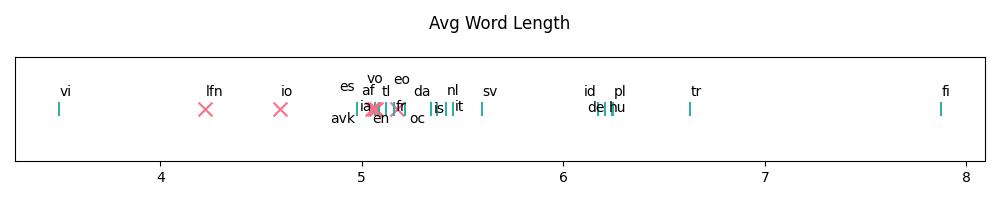
\includegraphics[width=\textwidth]{1d_Avg_Word_Length.png} 
  % \caption{Avg Word Length}
  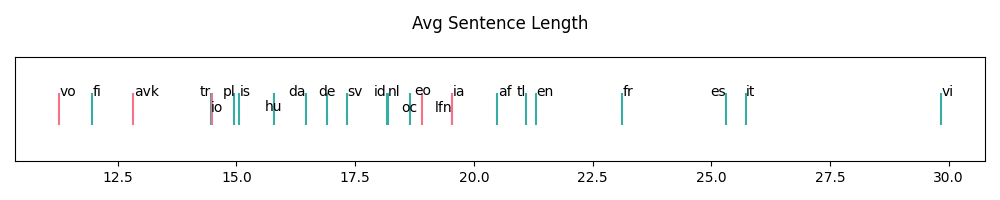
\includegraphics[width=\textwidth]{1d_Avg_Sentence_Length.png}
  % \caption{Avg Sentence Length}
  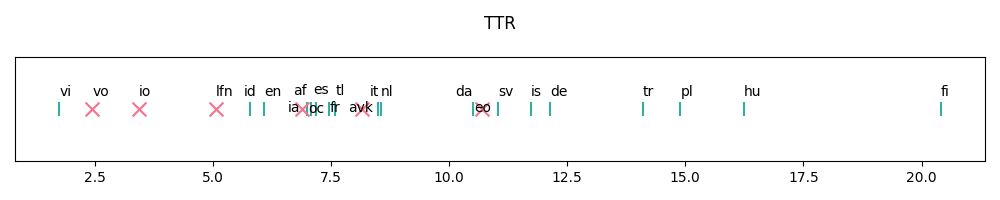
\includegraphics[width=\textwidth]{1d_TTR.png}
  % \caption{TTR}
  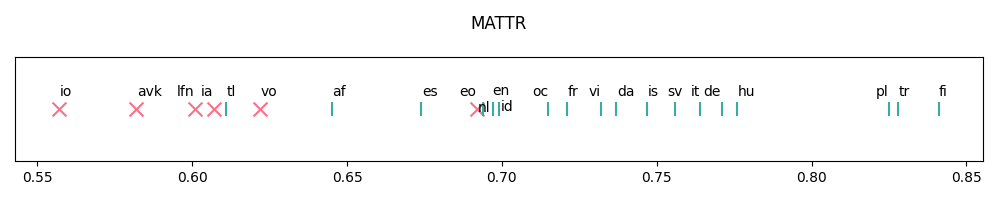
\includegraphics[width=\textwidth]{1d_MATTR.png}
  % \caption{MATTR}
  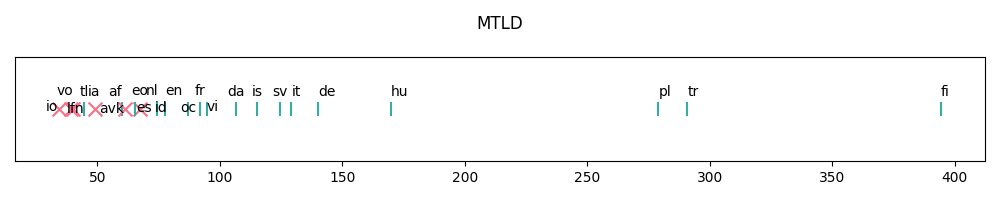
\includegraphics[width=\textwidth]{1d_MTLD.png}
  % \caption{MTLD}
  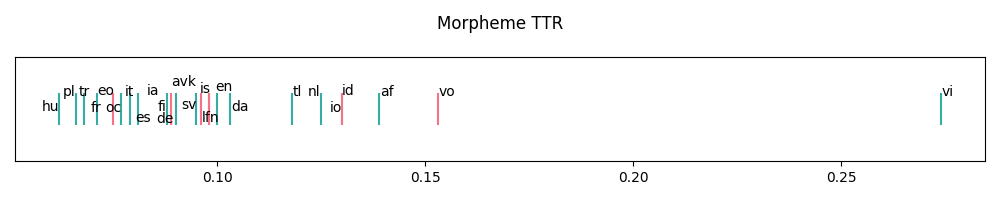
\includegraphics[width=\textwidth]{1d_Morpheme_TTR.png}
  % \caption{Morpheme TTR}
  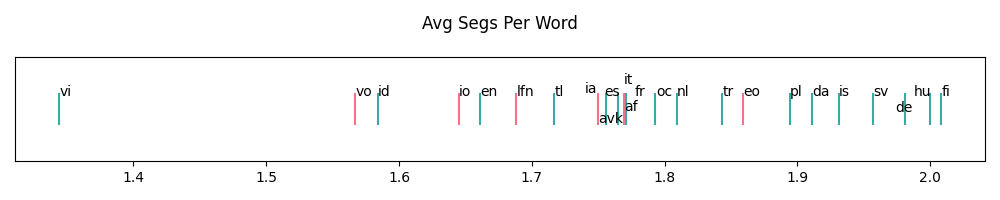
\includegraphics[width=\textwidth]{1d_Avg_Segs_Per_Word.png}
  % \caption{Avg Segs Per Word}
  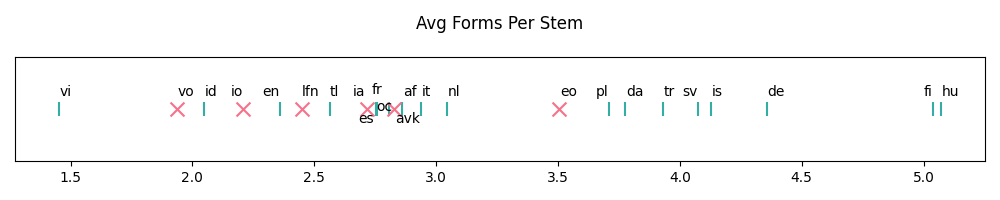
\includegraphics[width=\textwidth]{1d_Avg_Forms_Per_Stem.png} 
  % \caption{Avg Forms Per Stem}
\end{figure}

\clearpage

\begin{figure}[!ht]
  \centering
  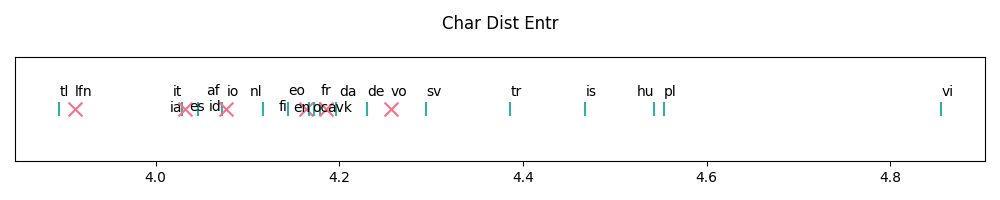
\includegraphics[width=\textwidth]{1d_Char_Dist_Entr.png}
  % \caption{Char Dist Entr}
  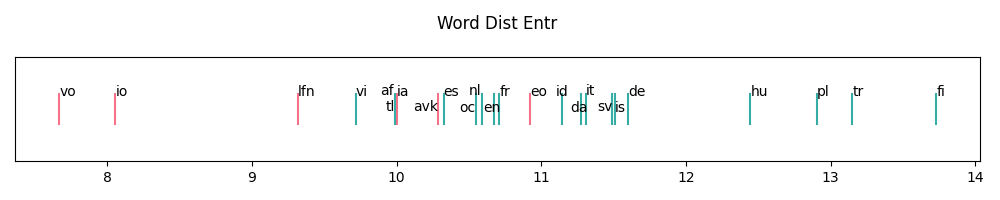
\includegraphics[width=\textwidth]{1d_Word_Dist_Entr.png}
  % \caption{Word Dist Entr}
  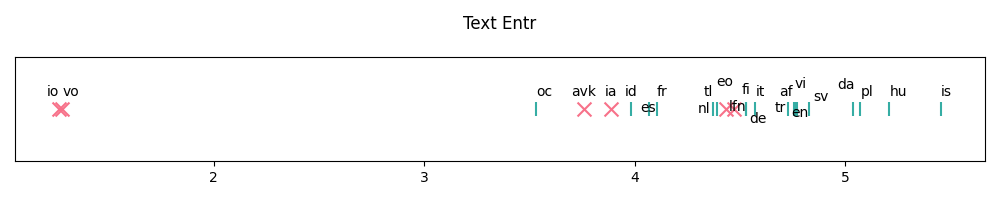
\includegraphics[width=\textwidth]{1d_Text_Entr.png}
  % \caption{Text Entr}
  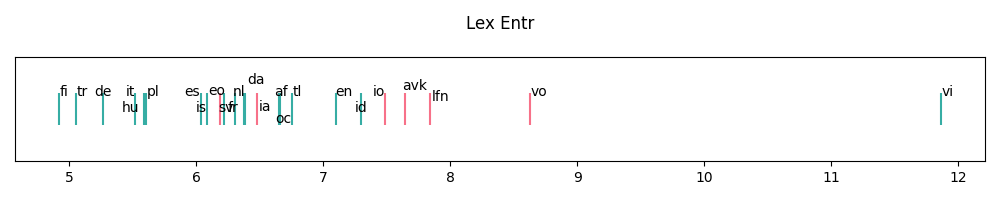
\includegraphics[width=\textwidth]{1d_Lex_Entr.png}
  % \caption{Lex Entr}
  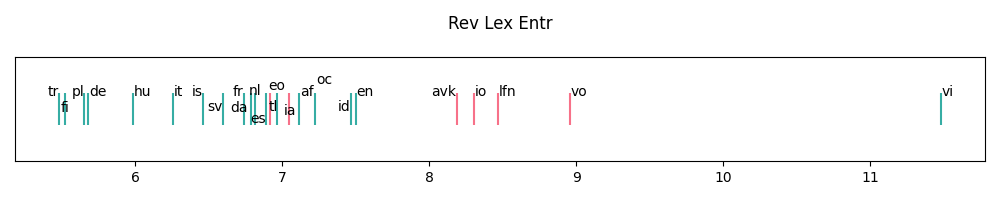
\includegraphics[width=\textwidth]{1d_Rev_Lex_Entr.png}
  % \caption{Rev Lex Entr}
  \caption{One-Dimensional Plots for Feature Distributions}
  \label{fig:1dfeatures}
\end{figure}

% \newpage

In the last group of features, corresponding to the five measurements of entropy, interesting patterns of clustering and imbalanced distributions again emerge in the findings. For character distribution entropy, the constructed languages are again grouped together on the left side. Perhaps unsurprisingly, given the exceedingly large size of its alphabet (i.e., the 93 lowercase alphabetical characters that comprise its corpora, a number which includes all variations of diacritics), Vietnamese is the highest value. Interestingly, though, this is followed next by Polish, despite having an alphabet size that is lower than several other languages in the study, suggesting the influence of other factors as well (e.g., orthography). On the other end of the spectrum is Tagalog with the lowest character distribution entropy, followed closely by Lingua Franca Nova.

In contrast, the measurements for word distribution entropy and text entropy both produced rather different results; rather than having a cluster on the left side, one appears in the center and right side, respectively. In both cases, Volapük and Ido have the lowest values, and in the latter case for text entropy, they are significantly lower than those of the other languages. As entropy is essentially a measure of predictability, this may be surmised as reflecting Volapük's intentional design of high regularity, especially with regard to morphology. The same can be said of Ido, though this along with comparison to the findings of the other constructed languages will be explored further in Chapter \ref{sec:discussion}. 

Last are the measures for lexical and reverse lexical entropy, which have very similar distributions. Vietnamese again emerged at one end of the spectrum with the highest entropy value, while agglutinative languages such as Finnish and Turkish appear at the opposite end with the lowest. Perhaps the most interesting finding here, however, is the cluster of constructed languages near the center of both distributions---with the notable absence of Interlingua and Esperanto, who instead appear in the midst of the natural languages on the left side in both cases.

% % Include table showing number of tokens and types for each language, together with the ratio calculation


\subsection{Results of PCA}
\label{ssec:pcaresults}

% PC1: TTR
% PC2: character distribution entropy
% PC3: average sentence length

% [DELETED] As a simplified explanation, this can be understood to mean that a language which has a high TTR and low reverse lexical entropy would have a high PC1 score. Looking at Figure \ref{fig:pcaanalysis} again, 
% [DELETED] Each principal component is therefore derived from a weighted combination of the features, with the loadings denoting the weights.

\begin{figure}[!h]
  \centering
  \caption{PCA Variance Screeplot - Kaiser Criterion}
  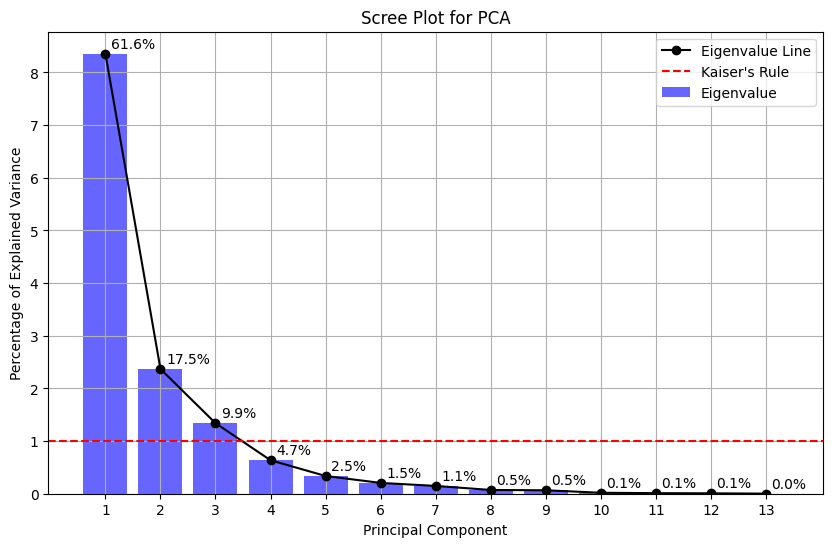
\includegraphics[width=0.7\textwidth]{PCA_Variance_Screeplot_kaiser.png}
  \label{fig:pckaiser}
\end{figure}

The result of applying the Kaiser criterion, shown in Figure \ref{fig:pckaiser}, identified three principal components which have eigenvalues greater than 1 and thus capture the most significant portion of the variance, which correspond to contributing to 61.6\%, 17.5\%, and 9.9\% of the total variance.

\begin{table}[!h]
  \centering
  \renewcommand{\arraystretch}{1.0}
  \begin{adjustbox}{width=\textwidth}
  \begin{tabular}{|l|l|l|l|l|l|l|l|l|l|l|l|l|l|}
  \hline
      ~ & \rotatebox{90}{\textbf{Avg Word Length}} & \rotatebox{90}{\textbf{Avg Sentence Length}} & \rotatebox{90}{\textbf{TTR}} & \rotatebox{90}{\textbf{MATTR}} & \rotatebox{90}{\textbf{MTLD}} & \rotatebox{90}{\textbf{Morpheme TTR}} & \rotatebox{90}{\textbf{Avg Segs Per Word}} & \rotatebox{90}{\textbf{Avg Forms Per Stem}} & \rotatebox{90}{\textbf{Char Dist Entr}} & \rotatebox{90}{\textbf{Word Dist Entr}} & \rotatebox{90}{\textbf{Text Entr}} & \rotatebox{90}{\textbf{Lex Entr}} & \rotatebox{90}{\textbf{Rev Lex Entr}} \\ \hline
      \textbf{PC1} & 0.312 & -0.152 & \textbf{0.343} & 0.271 & 0.284 & -0.25 & 0.318 & 0.328 & 0.042 & 0.323 & 0.19 & -0.305 & -0.319 \\ \hline
      \textbf{PC2} & -0.048 & 0.243 & 0.062 & 0.364 & 0.239 & 0.365 & -0.154 & 0.017 & \textbf{0.561} & 0.214 & 0.318 & 0.283 & 0.214 \\ \hline
      \textbf{PC3} & -0.232 & \textbf{0.671} & -0.075 & 0.02 & -0.237 & -0.175 & 0.045 & -0.06 & -0.263 & 0.099 & 0.511 & -0.171 & -0.168 \\ \hline
  \end{tabular}
  \end{adjustbox}
  \caption{Loadings for the top three principal components, with the most influential feature for each in bold.}
  \label{tbl:pcaloadings}
\end{table}

To interpret the degree to which each of the features in the data contributed to the formation of these dimensionally-reduced principal components, and therefore also determine the features that were the most influential (denoted in bold), the loadings are provided in Table \ref{tbl:pcaloadings}. Each loading indicates the magnitude of contribution to a feature, with positive or negative signs denoting the direction of influence (i.e., a positive loading means a positive correlation to the principal component, and vice versa). Thus, for example, the first principal component \textit{PC1} was most positively influenced by TTR and most negatively influenced by reverse lexical entropy, which have loadings of 0.343 and -0.319, respectively, and the next two overall most influential features following TTR were average forms per stem (0.328) and word distribution entropy (0.323). Similarly, for \textit{PC2}, the top contributing features were character distribution entropy (0.561), followed by morpheme TTR (0.365) and MATTR (0.364); for \textit{PC3}, these were average sentence length (0.671), text entropy (0.511), then character distribution entropy (-0.263).

\begin{figure}[!h]
  \centering
    \caption{Principal component analysis of the features using 2 principal components.}
    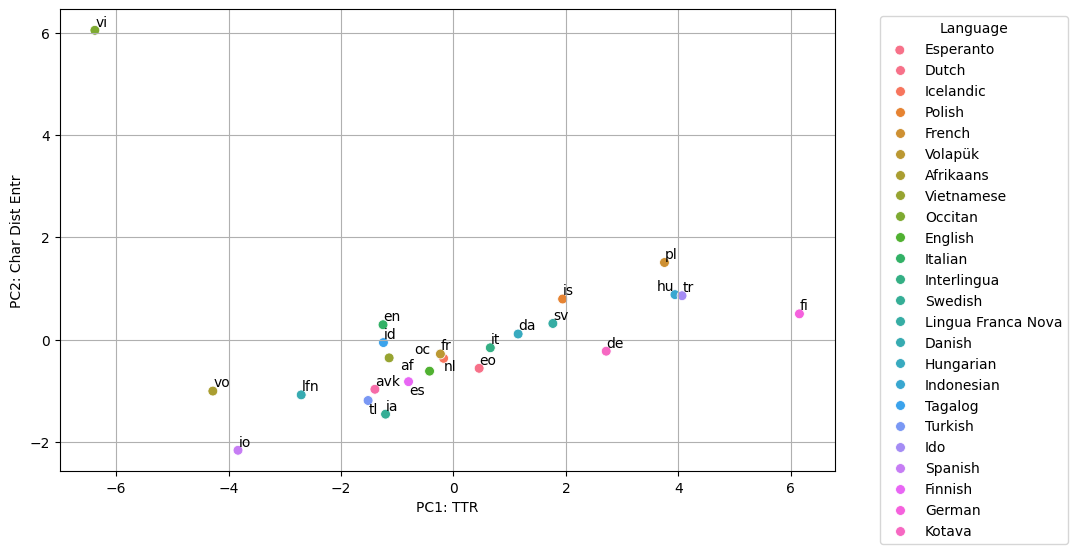
\includegraphics[width=1.0\textwidth]{PCA_of_Features.png}
    \label{fig:pcaanalysis}\
\end{figure}

Figure \ref{fig:pcaanalysis} shows the results of the dimensionality reduction performed on the data using PCA.\footnote{A script was used to increase the readability of the annotations in the graph: https://github.com/Phlya/adjustText} Note that since this is a two-dimensional diagram, it depicts only the top two principal components. The values along both axes denote the principal component scores. Additionally, the top influential feature for each, TTR and character distribution entropy, are also included in the axis labels for easier interpretation. 

Immediately noticeable in the diagram is the isolated position of Vietnamese at the top left, having the highest \textit{PC2} score and lowest \textit{PC1} score. Another interesting observation can be seen in the tight cluster of languages at the bottom center, to the left of which Volapük, Ido, and Lingua Franca Nova appear relatively close together. Another small cluster comprised of Polish, Hungarian, and Turkish is visible right of center, with Finnish appearing farthest on the right side. Overall, these findings---combined with the loadings shown in Table \ref{tbl:pcaloadings}---reiterate the previously discussed results in Section \ref{ssec:featureengineeringresults}.

% Include graph of explained variance following https://www.jcchouinard.com/pca-explained-variance/

\subsection{Results of Supervised Classification}
\label{ssec:classificationresults}

\begin{table}[!h]
  \centering
  \caption{Precision, recall, and F1-scores of the fine-tuned supervised binary classification models.}
  \renewcommand{\arraystretch}{1.0}
  \begin{tabular}{|l|l|l|l|}
  \hline
      \textbf{Model} & \textbf{F\textsubscript{1}-score} & \textbf{Precision} & \textbf{Recall} \\ \hline
      Decision Tree & 0.83 & 0.83 & 0.83 \\ 
      Random Forest & 0.83 & 0.83 & 0.83 \\ \hline
  \end{tabular}
  \label{tbl:supervisedevaluation}
\end{table}

As Table \ref{tbl:supervisedevaluation} shows, both classifiers achieved exactly the same precision, recall, and F\textsubscript{1}-scores. This comes as a bit of a surprise, since Random Forest is a comparatively more advanced model, but possible underlying reasons for this will be discussed in Chapter \ref{sec:discussion}.

\begin{figure}[!h]
  \centering
        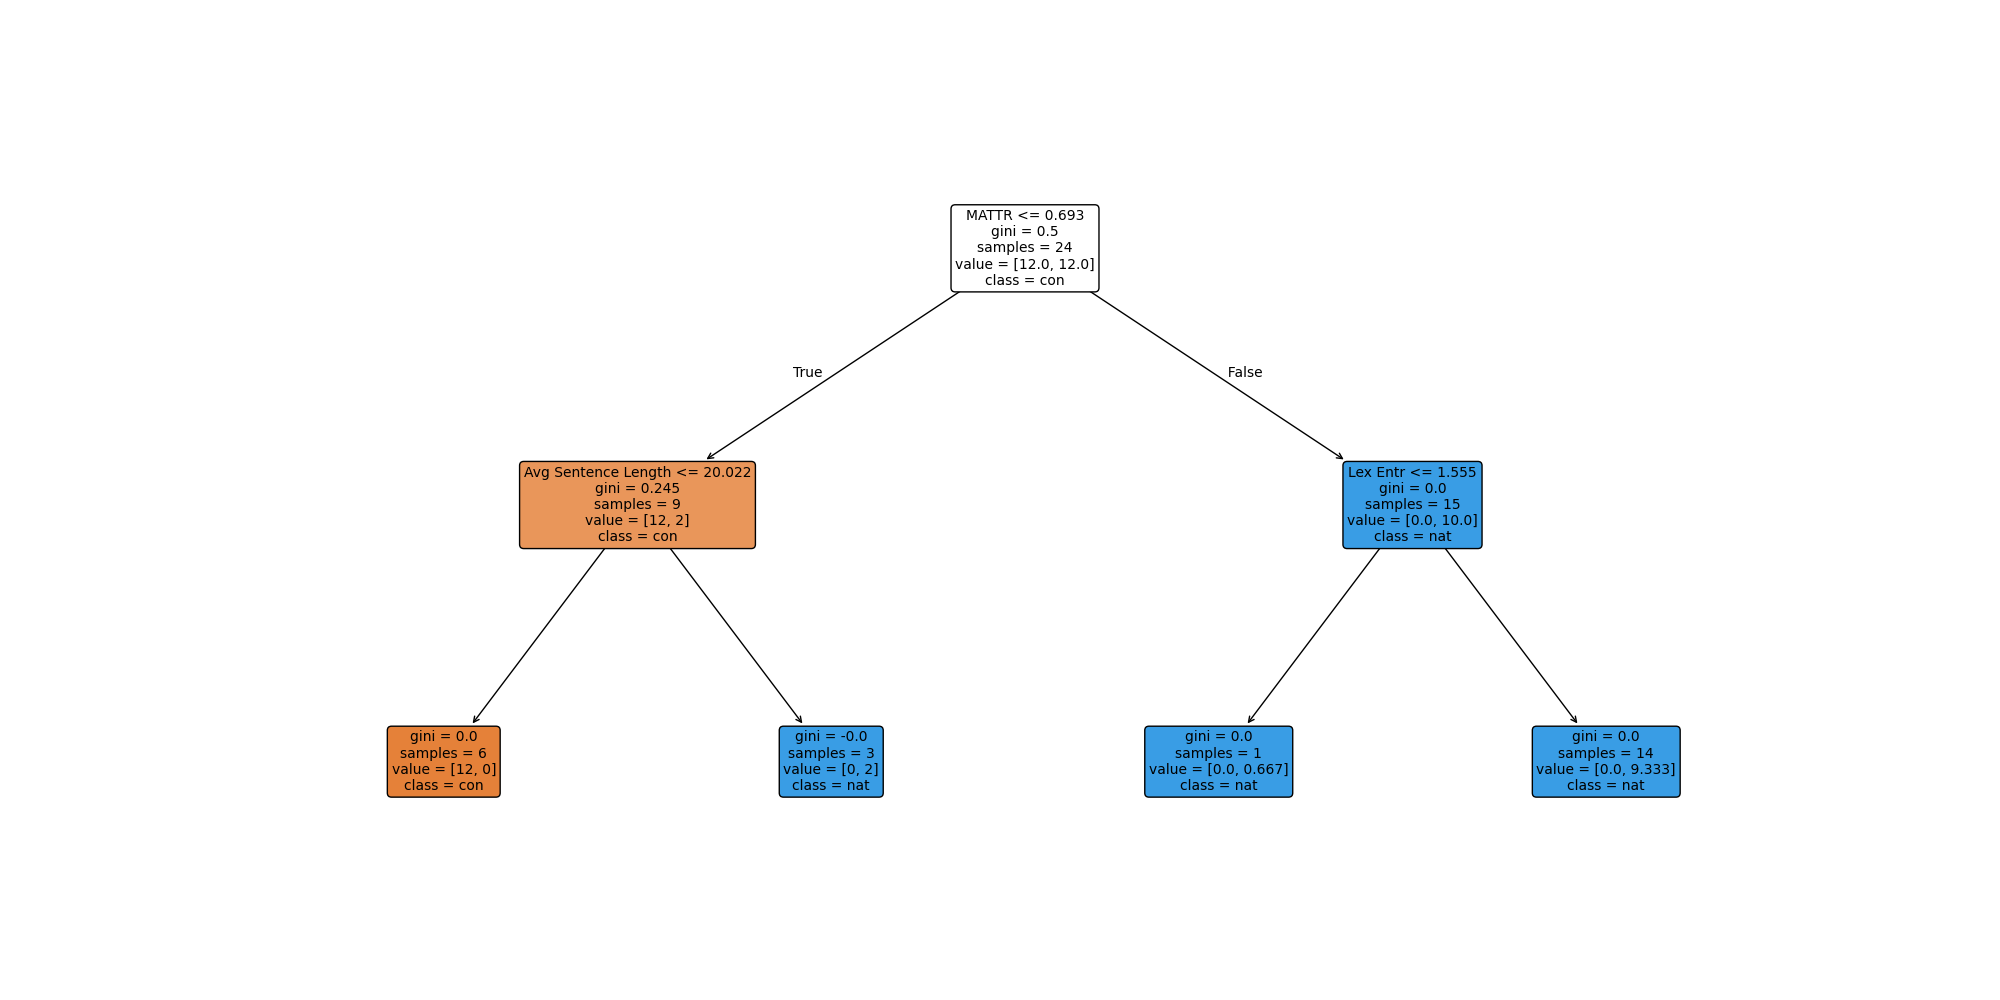
\includegraphics[width=1.0\textwidth]{decisiontree.png}
        \caption{Tree structure diagram for decision tree classifier}
        \label{fig:decisiontree}
\end{figure}

Figure \ref{fig:decisiontree} shows the resulting structure of the fine-tuned Decision Tree. To briefly explain how this is interpreted, for each node of the tree except the terminal ones, the top line is the condition for the subsequent split, and each split is a binary partition of the remaining number of samples. For example, the condition for the root node is \textit{MTLD} less than or equal to 70.824, which is true for 9 samples and false for the other 15. In addition, \textit{value} shows the weighted counts for both classes, with \textit{class} being equal to the majority class at that split, and \textit{gini} ranges from 0.0 (the samples all belong to one class) to 0.5 (the samples are evenly distributed, referred to as maximum impurity). Thus, the diagram indicates that the features MTLD, Average Sentence Length, and Average Word Length were the most discriminating features for this model's predictions. 

\begin{figure}[!h]
  \centering
  \begin{minipage}{0.5\textwidth}
    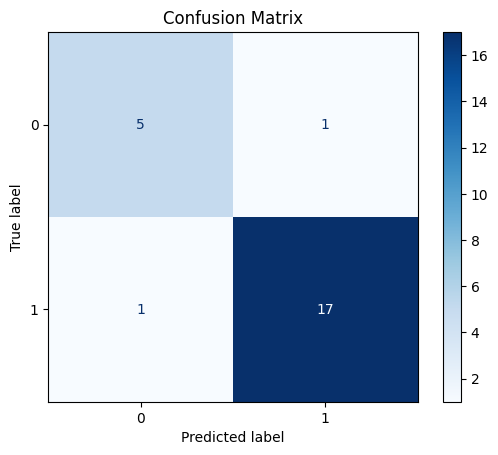
\includegraphics[width=\textwidth]{CM_decision_tree.png}
  \end{minipage}\hfill
  \begin{minipage}{0.5\textwidth}
    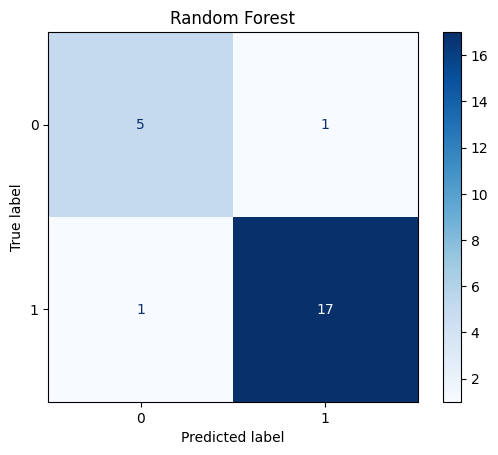
\includegraphics[width=\textwidth]{CM_random_forest.png}
  \end{minipage}
    \caption{Confusion matrices for the fine-tuned supervised binary classifiers: decision tree (left) and random forest (right).}
    \label{fig:cmsupervised}
\end{figure}

In the resulting confusion matrices for the fine-tuned supervised binary classifiers seen in Figure \ref{fig:cmsupervised}, the classes for \textit{constructed} and \textit{natural} correspond to 0 and 1, respectively, with constructed languages being the positive class. Both models made the same number of True Positive, False Positive, False Negative, and True Negative predictions. For the Decision Tree (left), Esperanto was incorrectly predicted as negative and Dutch incorrectly as positive. Similarly, the Random Forest (right) erroneously predicted Esperanto as negative too, but with Tagalog incorrectly as positive. This means, then, that both models mistakenly classified Esperanto as a natural language. 

\subsection{Results of Unsupervised Anomaly Detection}
\label{ssec:anomalydetectionresults}

\begin{table}[!h]
  \centering
  \caption{Precision, recall, and F\textsubscript{1}-scores of the fine-tuned unsupervised anomaly detection models.}
  \renewcommand{\arraystretch}{1.0}
  \begin{tabular}{|l|l|l|l|}
  \hline
    \textbf{Model} & \textbf{F\textsubscript{1}-score} & \textbf{Precision} & \textbf{Recall} \\ \hline
      Isolation Forest & 0.67 & 0.67 & 0.67 \\ 
      One-Class SVM & 0.73 & 0.80 & 0.67 \\
      Local Outlier Factor & 0.67 & 0.67 & 0.67 \\ \hline
  \end{tabular}
  \label{tbl:unsupervisedevaluation}
\end{table}

Table \ref{tbl:unsupervisedevaluation} shows the precision, recall, and F\textsubscript{1}-scores for the unsupervised anomaly detection models. The Isolation Forest and Local Outlier Factor achieved identical performance for precision, recall, and F\textsubscript{1}-scores, all of which were 0.67. On the other hand, despite also achieving the same score for recall, One-Class SVM performed slightly better in terms of precision and F\textsubscript{1}-score, with a score of 0.80 and 0.73, respectively.

\begin{figure}[!h]
  \centering
  \begin{minipage}{0.5\textwidth}
    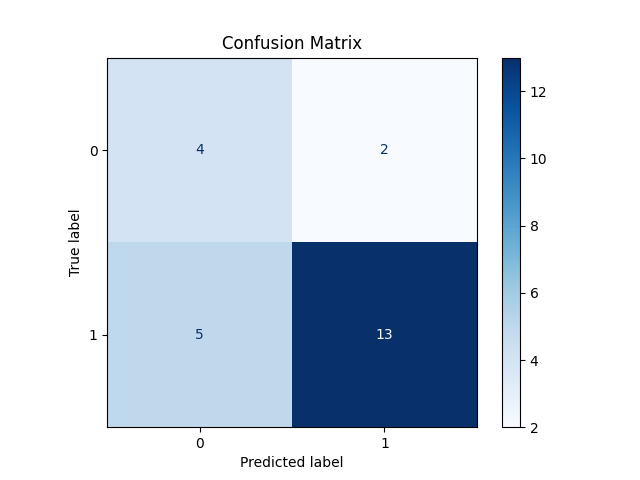
\includegraphics[width=\textwidth]{CM_ocsvm.png}
  \end{minipage}\hfill
  \begin{minipage}{0.5\textwidth}
    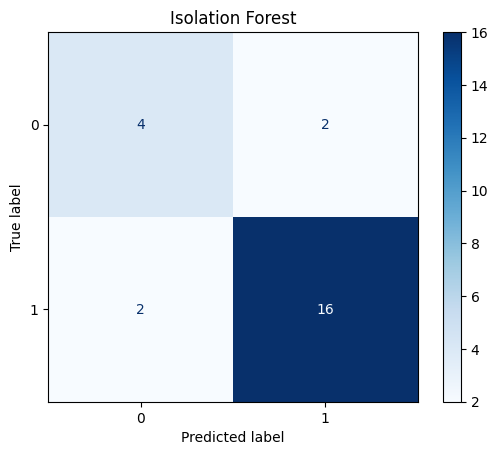
\includegraphics[width=\textwidth]{CM_if.png}
  \end{minipage}\par
  \vskip\floatsep
  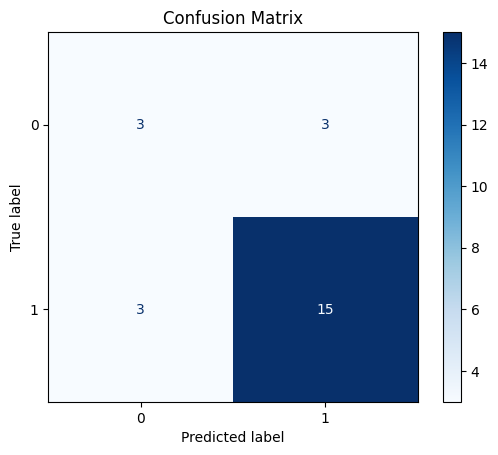
\includegraphics[width=0.5\textwidth]{CM_lof.png}
  \caption{Confusion matrices for the fine-tuned unsupervised anomaly detection models: one-class SVM (top left), isolation forest (top right), and local outlier factor (bottom).}
  \label{fig:cmunsupervised}
\end{figure}

The resulting confusion matrices for all three unsupervised models are provided in Figure \ref{fig:cmunsupervised}. Here again, constructed languages are the positive class being predicted, with 0 and 1 representing the constructed and natural language samples, respectively. 

Overall, the unsupervised models performed comparable to one another, with all three correctly predicting 4 positive instances. Regarding their erroneous predictions, the One-Class SVM falsely considered Esperanto and Interlingua to be negative, or natural languages, and Vietnamese as positive, or a constructed language. Interestingly, both the Isolation Forest and Local Outlier Factor models made exactly the same errors, with the addition of incorrectly predicting Finnish to be a positive instance in both cases too.

% \begin{figure}[!h]
%   \centering
%     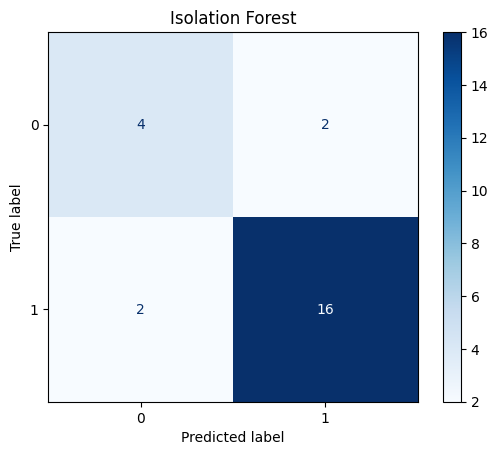
\includegraphics[width=0.5\textwidth]{CM_if.png}
%     \caption{Confusion Matrix for Isolation Forest}
%     \label{fig:cmisolationforest}
% \end{figure}

% \begin{figure}[!h]
%   \centering
%     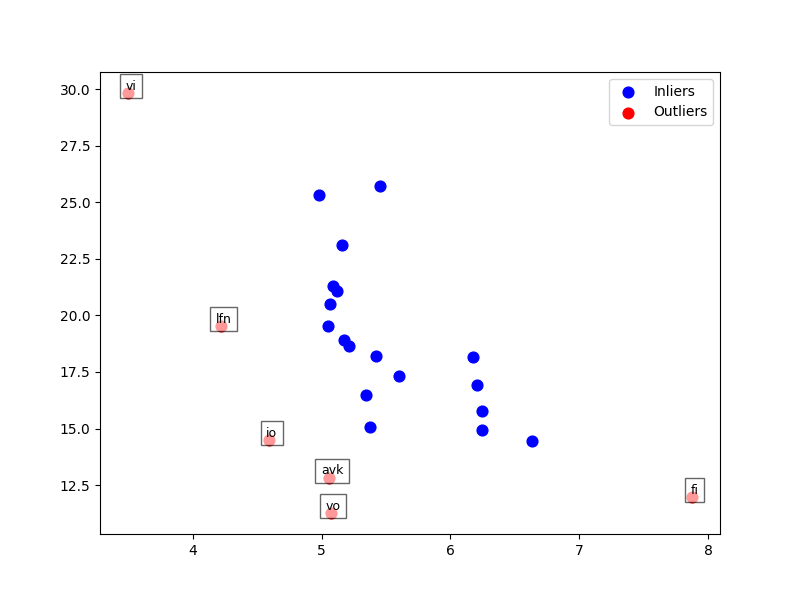
\includegraphics[width=0.5\textwidth]{IF_outliers.png}
%     \caption{Anomalies Detected by Isolation Forest}
%     \label{fig:isolationforestanomalies}
% \end{figure}

% \begin{figure}[!h]
%   \centering
%     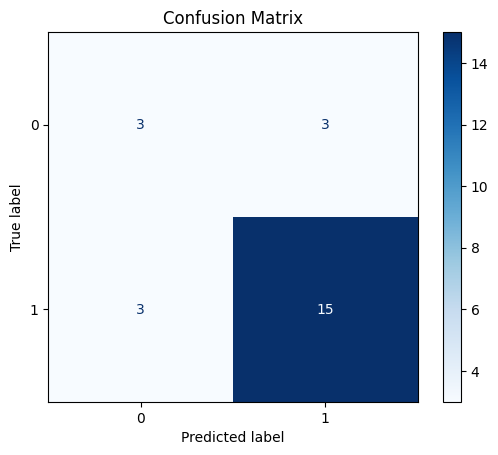
\includegraphics[width=0.5\textwidth]{CM_lof.png}
%     \caption{Confusion Matrix for Local Outlier Factor}
%     \label{fig:cmlof}
% \end{figure}

\subsection{Results of SHAP}
\label{ssec:shapresults}

% [DELETED] In some aspects, interpretation of the results of applying SHAP bears some resemblance to that of the PCA in Section \ref{ssec:pcaresults}; however, a key difference is 
% [DELETED] therefore, the horizontal distribution of said points corresponds to the level of variation that exists for that feature's influence on the model (i.e., a wide horizontal spread of points means the feature's influence on model predictions is highly variable across observations, and a cluster signifies the opposite)

The results of the Kernel SHAP method are visualized in beeswarm plots for global analysis, which are explained how to read here. The features, ranked in descending order according to their importance, comprise the y-axis. The x-axis, centered on zero (0.0), corresponds to SHAP values---measurements of the impact that a particular instance had on model prediction, represented in terms of magnitude and either positive or negative. Finally, the color coding spectrum represents the value of that instance, with the highest values denoted by red and the lowest ones denoted by blue.

\begin{figure}[!h]
  \centering
  \begin{minipage}{0.5\textwidth}
    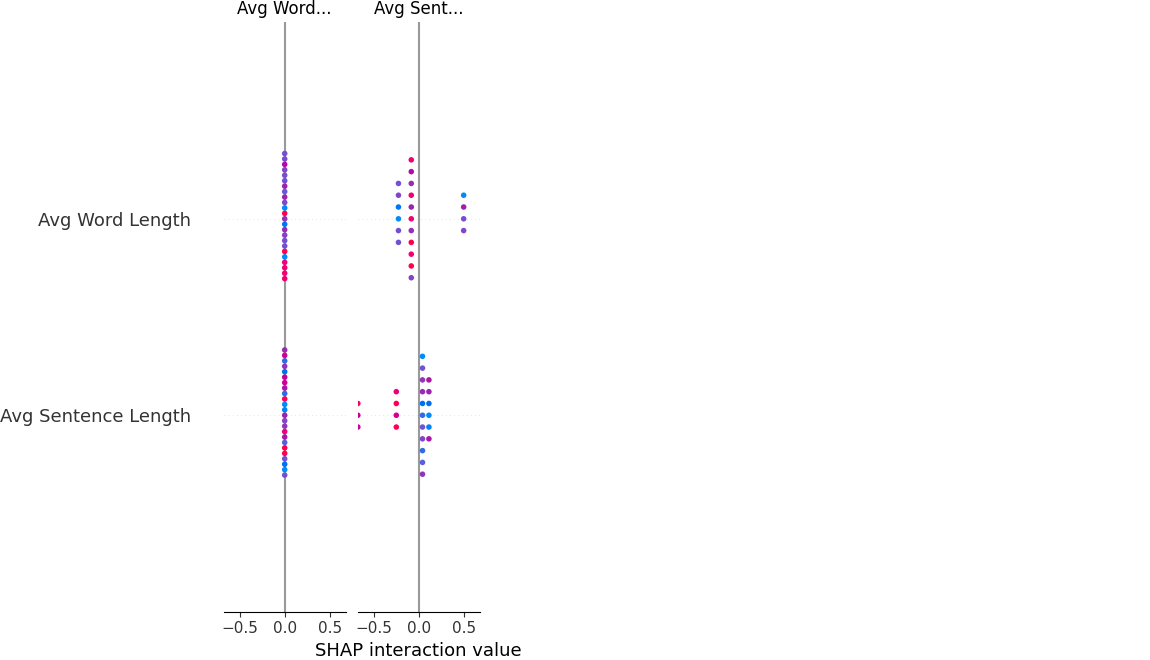
\includegraphics[width=\textwidth]{DT_SHAP_values.png}
  \end{minipage}\hfill
  \begin{minipage}{0.5\textwidth}
    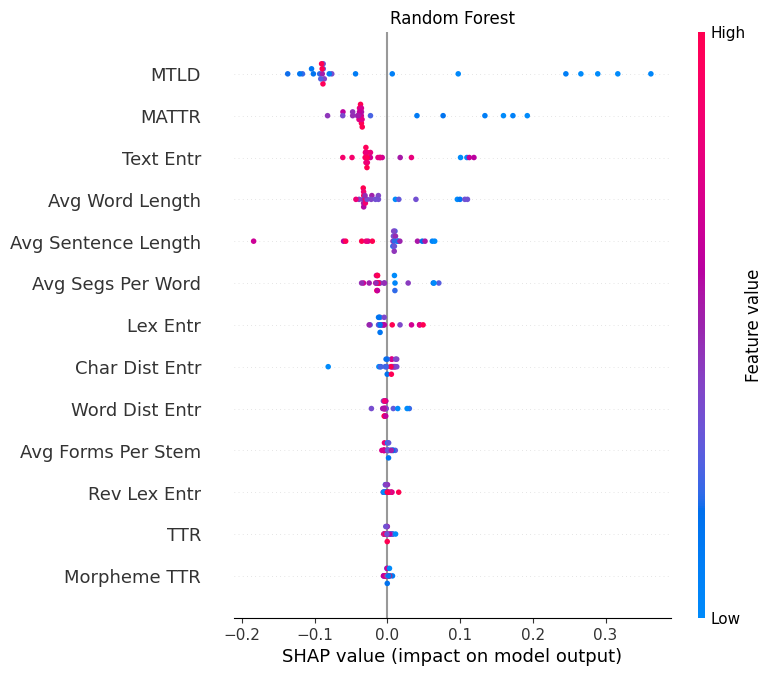
\includegraphics[width=\textwidth]{RF_SHAP_values.png}
  \end{minipage}
    \caption{Beeswarm plots for SHAP results on fine-tuned supervised models: decision tree (left) and random forest (right).}
    \label{fig:supervisedshap}
\end{figure}

Figure \ref{fig:supervisedshap} shows the two beeswarm plots corresponding to the supervised classifiers. Positive SHAP values correlate to constructed languages, and negative SHAP values correlate to natural languages. For the decision tree, only two features had any impact on the model's predictions: MTLD and average sentence length. Low values of the former correlated to a stronger positive impact, while high values of the latter correlated to a stronger negative impact. Notably, this also coincides with the findings shown by the tree structure diagram in Figure \ref{fig:decisiontree}. For the random forest, MTLD was again the most important, with lower values again correlating to having a stronger positive impact, followed by MATTR with the same correlation to a lesser extent. In contrast to the decision tree though, average word length was a less important feature here, and the random forest utilized a broader selection of features for its predictions overall. However, the clustering around zero shown by impacts for word distribution entropy, average forms per stem, reverse lexical entropy, TTR, and morpheme TTR suggest these features had very little influence on the random forest's predictions.

\begin{figure}[!h]
  \centering
  \begin{minipage}{0.5\textwidth}
    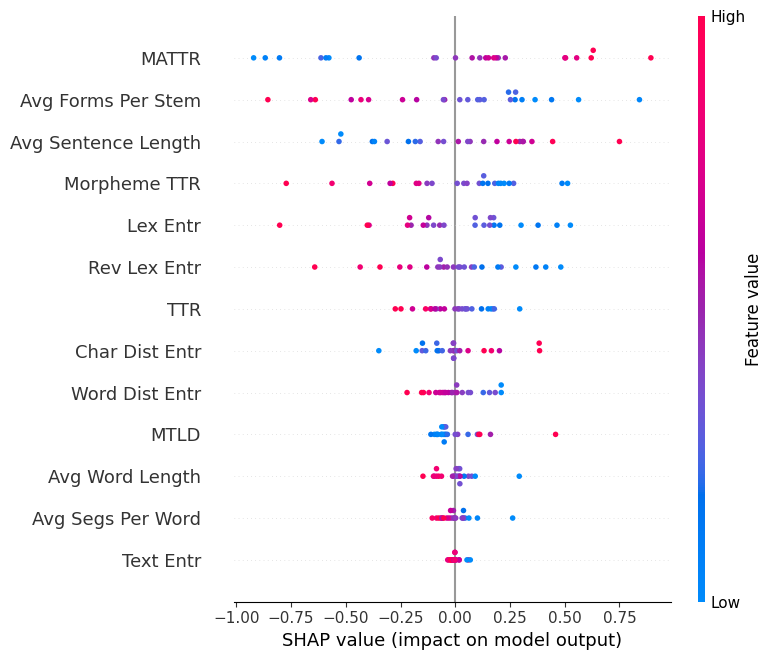
\includegraphics[width=\textwidth]{OCSVM_SHAP_values.png}
  \end{minipage}\hfill
  \begin{minipage}{0.5\textwidth}
    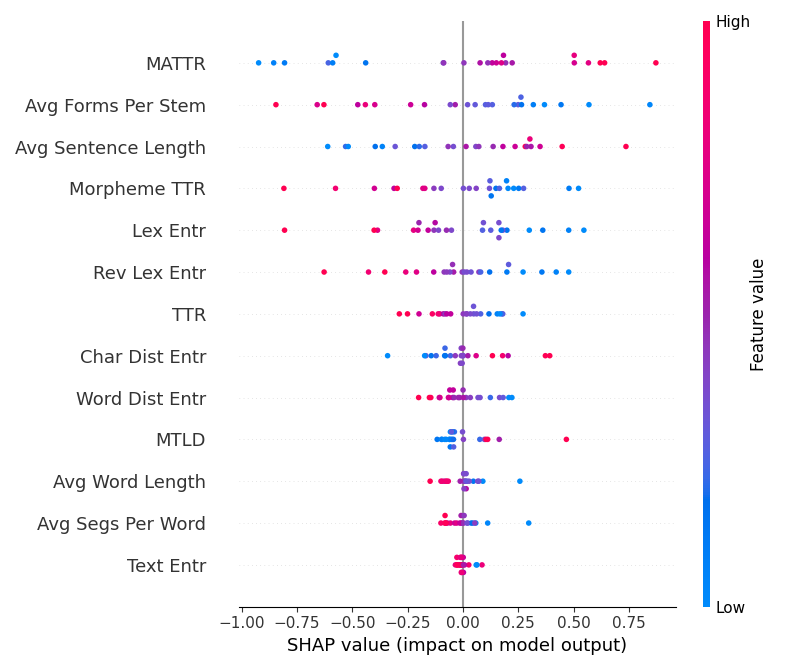
\includegraphics[width=\textwidth]{IF_SHAP_values.png}
  \end{minipage}
    \caption{Beeswarm plots for SHAP results on fine-tuned unsupervised models: one-class SVM (left) and isolation forest (right).}
    \label{fig:unsupervisedshap}
\end{figure}

The beeswarm plots for the two analyzed unsupervised models are shown in Figure \ref{fig:unsupervisedshap}. As these correspond to anomaly detection, their interpretation is slightly different due to the way the models make predictions. A negative anomaly score indicates a predicted anomaly (constructed language); likewise, a negative SHAP value indicates the same. Therefore, the plots show that MATTR was the most important feature for both models, with mid to low feature values being predicted as anomalies, suggesting that this was the strongest indicator for detecting anomalies in the dataset. Additionally, average sentence length and lexical entropy were highly influential for both models as well, with low values for the former and high values for the latter indicating anomalies. However, when comparing these with the feature results in Table \ref{tbl:featurestable} and their corresponding distributions shown in Figure \ref{fig:1dfeatures}, some possible discrepancy appears too. Namely, the second most influential feature for the one-class SVM, average forms per stem, shows that high feature values were seemingly indicative of an instance being a constructed language---contradictory to what the feature results shows. Potential reasons for this will be explained further in Chapter \ref{sec:discussion}.

% \begin{figure}[!h]
%   \centering
%   \begin{minipage}{0.5\textwidth}
%     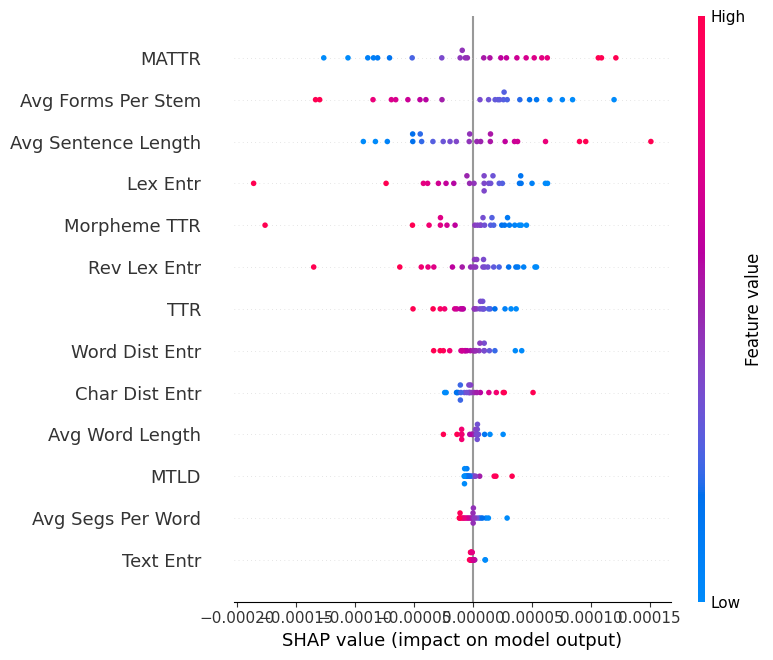
\includegraphics[width=\textwidth]{OCSVM_SHAP_granular.png}
%   \end{minipage}\hfill
%   \begin{minipage}{0.5\textwidth}
%     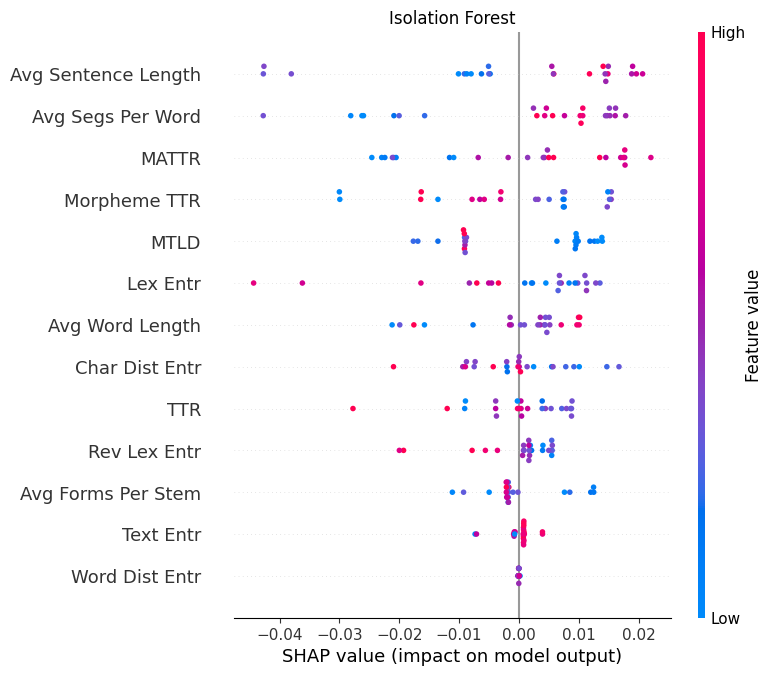
\includegraphics[width=\textwidth]{IF_SHAP_granular.png}
%   \end{minipage}
%     \caption{Beeswarm plots for granular SHAP results on fine-tuned unsupervised models: one-class SVM (left) and isolation forest (right).}
%     \label{fig:unsupervisedgranularshap}
% \end{figure}

% Lastly,

\clearpage
\newpage
\section{Discussion}
\label{sec:discussion}

% No early stopping implemented in PyTorch LSTM for calculating text entropy...
% Mention expectations (e.g. the conlangs coming from European languages, so the models might confuse these with the natural languages when classifying the two) and how they compare to the results
% Come back to the question/topic of linguistic universals, how do these results fit into the debate?
% Discuss problems with morphological complexity analysis: lack of gold standard corpus to evaluate models' segmentations, etc
% Compare the results of this task with those of classification of the raw text data (without the feature engineering, and using larger models like BERT), how the task and results might look different
% Using different window length for MATTR....
% Lack of validation for pytorch RNN (text entropy)
% [DELETED] linking back to the motivation and goals of this investigation as stated in the beginning of this thesis too.

% exhaustive analysis of every detail in the results not possible, but I will attempt to cover the most import parts

This section begins by revisiting the results of the feature engineering more in-depth, particularly the feature distribution plots from Figure \ref{fig:1dfeatures}, and then connecting these to the findings of the PCA, supervised classifiers, unsupervised anomaly detection models, and SHAP analysis to holistically address the primary focus of this thesis---comparing constructed and natural language---as well as address whether or not these findings align with initial expectations. In doing so, the potential linguistic implications of the results will be examined, along with possible explanations for observed patterns and discrepancies. Furthermore, some methodological shortcomings in the approaches used, and how these may have also impacted the final results, will also be noted.

Analyzing the feature distributions plots shown in Figure \ref{fig:1dfeatures} again, it is evident that, out of all languages in the dataset---both constructed and natural---Vietnamese and Finnish consistently appear as the most extreme instances for many of the linguistic features measured, often having either the lowest or highest values. There are some notable exceptions to this, though; for instance, while Vietnamese has the lowest value for TTR, it is closer to the median of the distributions for MATTR and MTLD. In comparison, Ido has a low value for TTR as well, being only slightly higher that of Vietnamese (and Volapük). However, Ido has the lowest MATTR and MTLD values; in fact, all of the constructed languages have lower values for MATTR and MTLD than not only Vietnamese, but most of the other natural languages in the dataset too, outside of a few exceptions---a point we will return to when discussing the classifiers and anomaly detection models. As noted previously, in the case of Vietnamese, having the lowest TTR (and indeed, having the lowest or highest values for other features too) might be explained simply by way of its highly isolating and monosyllabic morphology---being an extremity in the dataset in that regard---which consequently tends to result in more frequent repetition of certain vocabulary, such as when forming compound words. In contrast to TTR, MATTR and MTLD are able to capture more changes in lexical variation throughout a text (and are irrespective of overall text length) due to how they are calculated. Thus, they are less affected by lower counts of unique words (types) for an entire text. In a similar vein, this could also explain why the same drastic change in position within these distributions is not observed for many of the other natural languages in the dataset that have more complex morphologies in comparison (e.g., Swedish, Icelandic, German, Hungarian, Polish, Turkish, and Finnish), and thus a general tendency for less repetition and more unique word formation, as any lexical richness captured using the simple metric of TTR would likely still be observable even at a more granular level with MATTR and MTLD.

Regarding constructed languages within these three distributions, there is a clear general pattern of having lower values compared to the natural languages, which could be attributed to several different underlying reasons. The first---which is actually more widely applicable to all of the language data and will be a recurring notion throughout this chapter---is the quality of the text data itself. In addition to the apparent prevalence of low-quality machine translations for, at the very least, Volapük's Wikipedia entries that was already noted in Section \ref{ssec:wikimedia}, the often niche communities of speakers of constructed languages---the least of which being Esperanto---makes it likely that much of the Wikipedia data for them was written by a small number of people. Consequently, this can limit lexical diversity. Another possible explanation, and indeed the focal point of this thesis's investigation, stems from the design of the constructed languages themselves. Being IALs, they were, generally speaking, created to be more regular in various linguistic aspects than their natural counterparts---some even more so than others. For instance, Ido was essentially designed to be a more regular version of Esperanto, including lexically, which may explain it having much lower values for lexical diversity compared to Esperanto despite being directly derived from it. Similarly, having a relatively fixed lexicon---that is, a vocabulary that is not changing much over time, as is instead usually the case for natural languages---may be a factor here as well.

In the case of Finnish, a notable exception to this pattern of appearing as an extreme instance for the different feature values is, maybe surprisingly, in the distribution for morpheme TTR. Whereas it is one of the highest values for both of the other two measurements of morphological complexity, it instead appears closer to the median for this one, with Hungarian---who is from the same language family (Uralic) as Finnish---having the lowest. Even more shockingly, Finnish has an even higher morpheme TTR than Esperanto. Since this measurement is the ratio of unique morphemes to total morphemes in a text, one might infer then that Finnish tends to utilize a greater number of unique morphemes in its constructions than other languages like Hungarian. Another possible explanation for this discrepancy may also be from the unsupervised segmentation models used for calculating morphological complexity; due to limitations (such as the inclusion of many low-resource languages in the dataset), the precision and recall of the models' segmentations for each language could not be adequately evaluated with ease. Therefore, this could also merely be an error in the segmentations for Finnish. Conversely, it could be that the measurement for Finnish is correct and those of the other languages are erroneous instead; the segmentation model that was used is an implementation written by researchers in Finland, \textcite{Smit2014inproceedings}, which lends credence to this possibility to some degree. However, determining the exact cause with more certainty would require deeper investigation. 

Additional points worth mentioning include the extreme similarity of the other two feature distributions (more specifically, the order of the languages) for morphological complexity, average number of segmentations per word and average number of forms per stem. As they are both essentially measuring the same underlying morphological processes, just in slightly different ways, this resemblance is not a complete surprise, and it may suggest that the inclusion of both features is actually redundant. However, as we will see shortly when discussing the results of the SHAP analysis, this also might not necessarily be the case. Lastly, when specifically examining the constructed languages within the three distributions, they appear to have less of an overall separation from the natural languages compared to other features like MATTR, MTLD, or lexical entropy. That being said, there are also some consistent and familiar patterns; Esperanto again appears as the most extreme case out of the constructed languages, having the lowest morpheme TTR and highest average number of forms per stem and average number of segmentations per word of the six---values which are relatively comparable to many of the natural languages. Furthermore, Volapük was consistently on the opposite end of the spectrum from Esperanto each time (closely followed again by Ido); it is difficult to say, though, the degree to which this accurately reflects expectations based on prior research and understanding of Volapük's morphological structure, or is in fact another possible discrepancy in the results. According to \textcite{Reagan2019book}, Volapük is an agglutinative language described as being grammatically and morphologically complex, a description that seems understated in the face of claims of having upwards of 1,584 ways to conjugate a verb \parencite{Reagan2019book,Rogers2011book}. As such, its high morpheme TTR would suggest this complexity is expressed using a relatively high number of unique morphemes. At the same time, though, the low values for average number of segmentations per word and average number of forms per stem arguably appear, on the surface, contradictory to this characterization, especially when compared to strongly agglutinative languages in the dataset like Hungarian and Finnish. % come  back to this

% [DELETED] The last of the feature distributions to examine are the various measurements for entropy.

As was already mentioned in Section \ref{ssec:featureengineeringresults} regarding character distribution entropy, at first glance it appears to have some degree of correlation to the number of unique alphabetical characters in a given language's corpus, as would be expected. Intuitively, the other likely biggest contributing factor is orthography. Tagalog, for example, has the lowest entropy value of all the languages, which could be due to its frequent use of consonant-vowel patterns, as seen in words like \textit{tarayan} (to be rude to someone), \textit{baka} (cow), and \textit{sala} (living room). Lingua Franca Nova being the lowest of the constructed languages could be in part explainable as reflecting its intended strict adherence to phonetic spelling; on the other hand, the same is also true for Kotava and (for the most part) Ido, yet the findings show Esperanto's entropy to be lower than Kotava's, and Interlingua lower than all three, so this interpretation is left inconclusive. As a whole, the relatively similar character distribution entropies of some of the constructed languages (namely Interlingua, Esperanto, Lingua Franca Nova, and Ido) and their close proximity with the Romance languages in the distribution fits prior expectations. 

As theorized already, high grammatical and morphological regularity may account for the isolation of both Volapük and Ido from the other languages for word distribution entropy and text entropy. Focusing on former of the entropy measures first, Volapük's result and its characterization as an agglutinative language again appear to be in contradiction 

% It is also important to mention the influence that the quality of the text data itself has on the resulting measurements for the features.

% Discuss with Schubert (1993) article
% Mention unexpected results about Kotava
% (optionally) mention mistake about excluding diacritics from Tagalog alphabet 

Additionally, Kotava's results are somewhat surprising here. Despite its intended \textit{a priori} design, it does not stand out in any of the feature distributions. In fact, out of all six constructed languages, it never appears as having the highest or lowest value for a feature, instead always being somewhere in the middle. While the quality of the corpus data could likely be the main underlying reason for these results, with most or all of it probably being written by a very small number of people---considering how niche the language is---it would also be interesting to see how much is actually due to the language itself. That is to say, if such dissimilarity to all other human languages is actually not as noticeable empirically when measured for morphological diversity, lexical diversity, or entropy.

Overall, constructed languages do not appear as distinct from the natural languages for the features as might have been initially expected, and in fact some natural languages---namely Vietnamese and Finnish---consistently stood out instead. These results were again illustrated in the PCA performed on the data, shown in Figure \ref{fig:pcaanalysis}, too. Even when some level of distinction was more clear, for example with MATTR, it did not include all constructed languages. In particular, and perhaps most interestingly, Esperanto often appeared to be comparable to many of the natural languages---a phenomenon that is seen again with the supervised and unsupervised models---and even more so than its peers in many cases. Whether this is a reflection of some aspects of Esperanto's original design resembling natural language, an indication of undergoing linguistic evolution and development which in turn produces more "natural" qualities, a result of having a larger community of speakers and thus more variety of contributors to Wikipedia---thereby making the corpus for Esperanto more robust, or still other reasons not considered here, it is difficult to conclude more concretely without further experimentation and data. 

% Without more investigation, however, only tentative conclusions can be drawn about the results.

% for morph complexity, models are not accurate, corpora text is not good (poor machine translations for conlangs)

% morpheme TTR and avg segs per word are flipped distributions, with some slight discrepancies that could be explained as caused by number of morphemes in language being different from number of unique morphemes

%  Interestingly, MATTR was the most important feature for both models, suggesting that it serves as a strong indicator for detecting anomalies in the dataset -> Explain further using other results too

% Note that the SHAP values are for model explainability, which is extrapolated to explain feature importance and infer broader conclusions about the linguistic nature of constructed/natural languages 

% IF SHAP - MTLD, char dist entr - the inliers (right side) all correspond to high values, very different than the 1d plot shows

\subsection{Models \& Feature Importance}
\label{ssec:modelsandfeatureimportance}

It bears repeating that due to the relatively small size of the dataset being used, conclusions derived from the results of the models are only tentative and in fact may not be exactly the same in the case of a larger dataset. For example, the measured precision, recall, and F\textsubscript{1}-scores of the models, while still providing useful insights, are not sufficient to conclusively determine broader implications about their overall level of success and are mostly not different enough from one another to analyze in more detail either beyond speculation. This can be seen in the case of the decision tree and random forest classifiers, which both have the same score for all three metrics despite model differences. With more data, such as the inclusion of more languages, these scores would likely be more informative. However, there were still some noteworthy observations from the models, as well as the SHAP analysis applied on them, that are of interest here.

The biggest of these was the reinforcement of the same aforementioned trends from the feature distributions in both the supervised classification and unsupervised anomaly detection, with Esperanto consistently failing to be considered a constructed language by all five models, and---in the case of anomaly detection specifically---difficulties with Vietnamese and Finnish as well. Even more interestingly, all three anomaly detection models also considered Interlingua to be a natural language. As Interlingua was designed to be closely resembling natural languages (specifically Romance languages) even to the point of intentionally introducing irregularities, as discussed in Section \ref{ssec:constructedlanguagesinthedataset}, this misclassification may be seen as its creators' goals having been successfully achieved. However, it is not exactly clear why this finding would appear for the anomaly detection models but not the random forest or decision tree. Likewise, the discrepancy between the one-class SVM correctly considering Finnish to be a natural language and the local outlier factor and isolation forest models mistakenly considering it constructed is also not immediately clear, although it could be inferred to potentially stem from the way the one-class SVM determines its decision boundary. % come back to this

Delving a bit deeper into analyzing the SHAP global feature importances shown in Figures \ref{fig:supervisedshap} and \ref{fig:unsupervisedshap}, lexical diversity was most discriminative for the four models analyzed in determining between natural and constructed languages, based on MTLD being the top influential feature for the supervised classifiers (decision tree and random forest) and MATTR being the top influential feature for the unsupervised anomaly detection models (isolation forest and one-class SVM). Measures of morphological complexity and entropy were also influential to different degrees, though varying widely across all models. For example, for the two anomaly detection models, lexical (and reverse lexical, in the case of the one-class SVM) entropy was the most influential of the entropy measurements. This is supportive of the respective distribution plots in Figure \ref{fig:1dfeatures}, which indeed show a clear separation between the constructed and natural languages---with the exception of Esperanto and Interlingua. However, these same two entropy features had very little influence on the random forest and essentially zero influence on the decision tree, potentially suggesting a difference in what are considered discriminative features for supervised classification versus unsupervised anomaly detection. Another possible explanation though could simply be that such differences are model-specific, and not actually reflective of the features themselves. Additionally, in the case of the decision tree specifically, MTLD and average sentence length appear as the only two features which influenced model predictions, and they also appear as the two biggest features (followed by average word length) selected for splits as shown in Figure \ref{fig:decisiontree}, suggesting a correlation between these two specific features and the discernibility of natural and constructed languages in the data. 

Feature importance at the global level for the isolation forest can be compared to a more localized context with individual observations, shown in the force plots in Figure \ref{fig:shapforceplots}. These plots provide an additive view of each feature and how it influences the final prediction of the model. Two natural (Finnish and English) and two constructed languages (Esperanto and Volapük) are given to demonstrate a correct and incorrect prediction for each.

\begin{figure}[!ht]
  \centering
  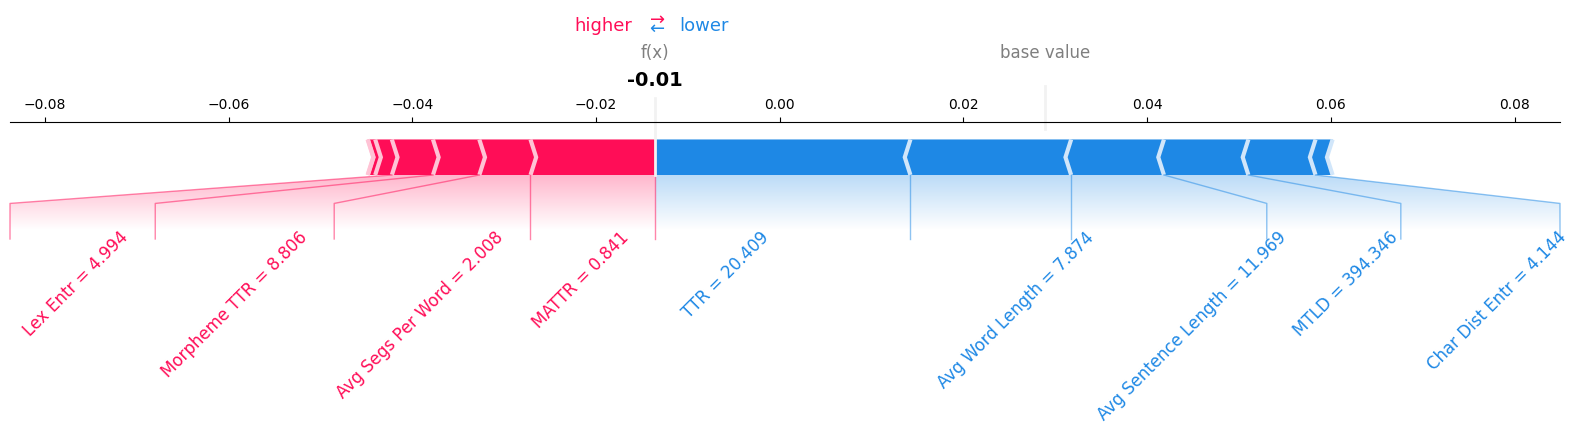
\includegraphics[width=\textwidth]{IF_SHAP_force_fi.png} 
  \caption{Isolation Forest - SHAP force plot for Finnish}
  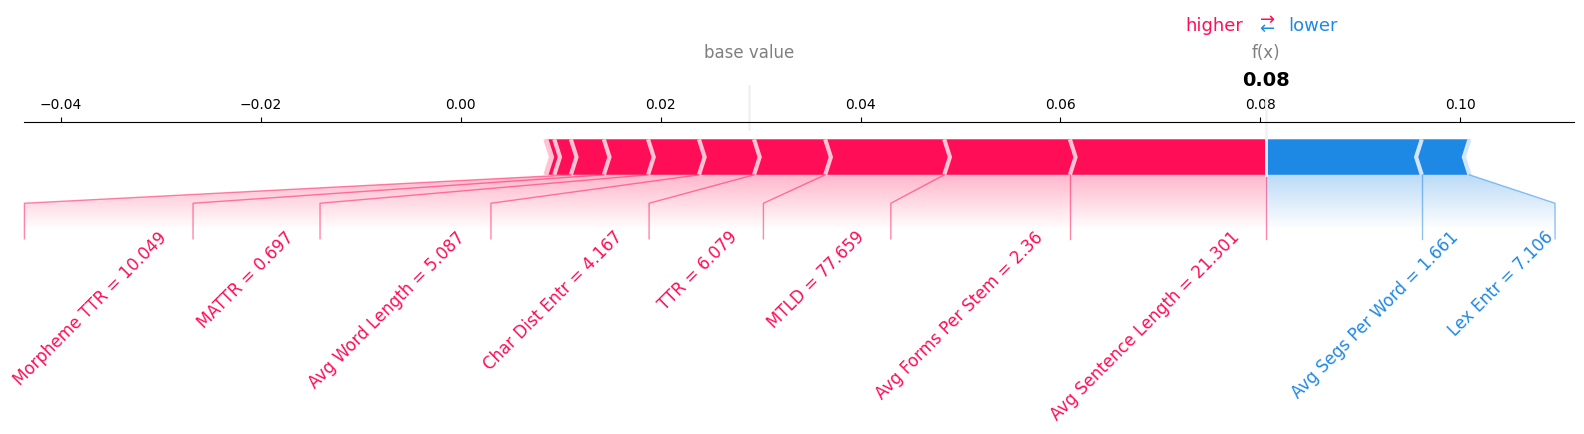
\includegraphics[width=\textwidth]{IF_SHAP_force_en.png}
  \caption{Isolation Forest - SHAP force plot for English}
  % 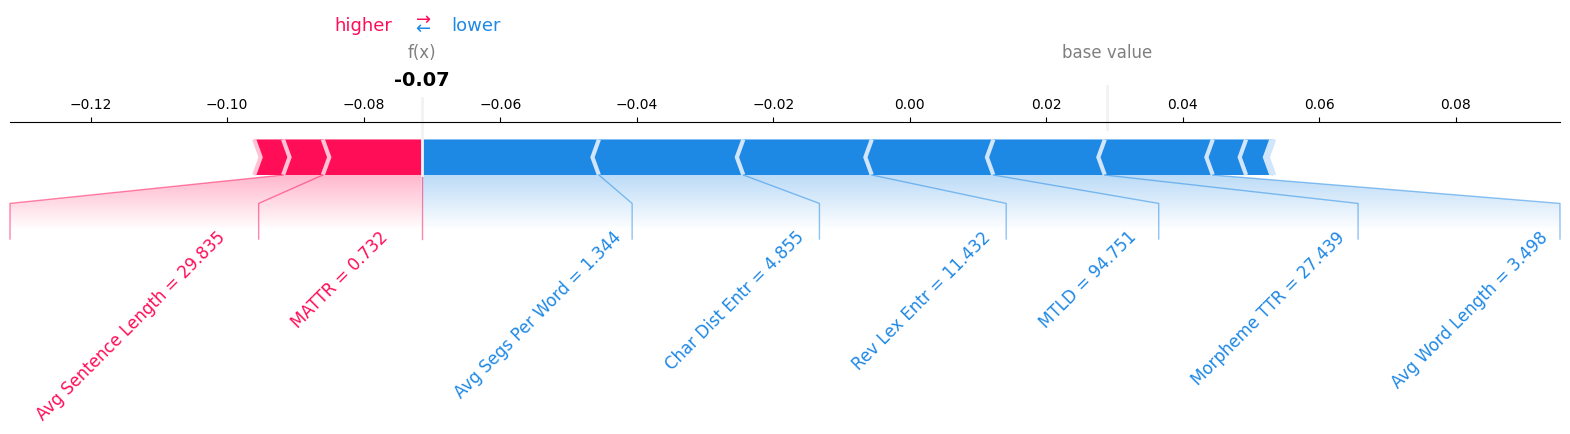
\includegraphics[width=\textwidth]{IF_SHAP_force_vi.png}
  % \caption{Isolation Forest - SHAP force plot for Vietnamese}
  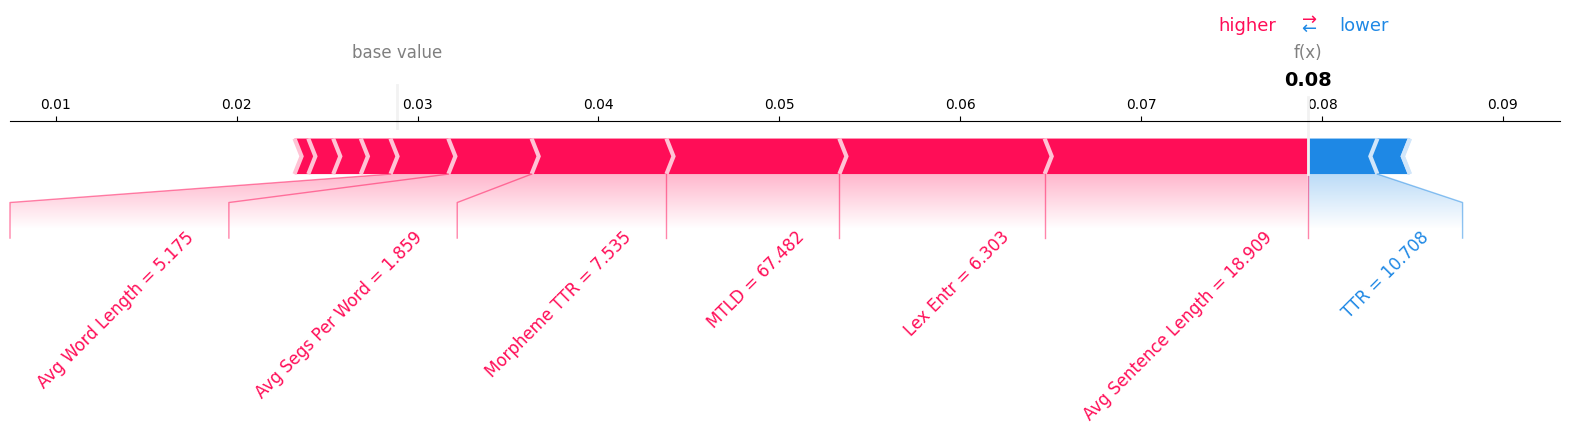
\includegraphics[width=\textwidth]{IF_SHAP_force_eo.png}
  \caption{Isolation Forest - SHAP force plot for Esperanto}
  \includegraphics[width=\textwidth]{IF_SHAP_force_vo.png}
  \caption{Isolation Forest - SHAP force plot for Volapük}
  % \includegraphics[width=\textwidth]{IF_SHAP_force_io.png}
  % \caption{Isolation Forest - SHAP force plot for Ido}
  \label{fig:shapforceplots}
\end{figure}

Here, we can 

\clearpage
\newpage
\section{Conclusion}
\label{sec:conclusion}



\subsection{Future Work}
\label{ssec:futurework}

The research presented in this thesis is far from encompassing all there is to the topic of defining language, and distinguishing between constructed and natural language. At present, this is an area of research with ample room for potential development. 

Limiting factors: number of languages and which languages/language families, lack of real parallel corpora, problems associated with low-resource languages, relatively narrow scope of experimentation,

\newpage
\section{Acknowledgments}
\label{sec:acknowledgments}

I would first and foremost like to thank my main supervisor, Dr. Çağrı Çöltekin, for all of his patience and support regarding this thesis, as well as my overall studies. All of his help and guidance has been invaluable to me, and I would not have been able to complete this otherwise. The same gratitude also extends to my other supervisor, Dr. Christian Bentz, for his interest and support regarding my research. Both of these incredible people were sources of encouragement for me when I most needed it, and for that I am extremely grateful. 

Additionally, I want to thank my friends and family who helped me at every step. Though I would not be able to name all of them here, I am especially grateful for the support from my good friends Fidan, Leixin, Selene, Linhong, Pascal, and Lisa, as well as from my siblings, parents, grandparents, and aunt. 

Though it may be less conventional, I also would like to thank my therapist and psychiatrist for all of their support and help too, not only with my thesis, but regarding all of my studies since I came here to Germany. It would not be an exaggeration to say that I was able to get this far because of them.

Last but not least, I want to sincerely thank my amazing girlfriend, Momoho, for her endless support, patience, care, and reassurance. She was a guiding light for me during this time, and I owe her a lifetime of gratitude for it.

\newpage
\begingroup
\sloppy
\printbibliography
\endgroup

\newpage
\section{Appendices}
\label{sec:appendices}

Here I...

\subsection{Corpora}
\label{ssec:corporaapp}

% Include number of symbols in the alphabet for each language? (Gomez 2014, Table 1)
% Include number of types/tokens?

\begin{table}[!h]
  \centering
  \renewcommand{\arraystretch}{1.5}
  \begin{tabular} {|p{3cm}|p{3cm}|p{3.5cm}|p{3.0cm}|}
  \hline
  \textbf{Language} & \textbf{Number of Words} & \textbf{Number of sentences} & \textbf{Alphabet Size} \\
  \hline
  Icelandic & 629995 & 41847 & 32 \\
  German & 629987 & 37261 & 30 \\
  Polish & 629997 & 42138 & 35 \\
  Ido & 629990 & 43496 & 26 \\
  Afrikaans & 629994 & 30737 & 43 \\
  Kotava & 617400 & 48145 & 29 \\
  Hungarian & 629946 & 39916 & 54 \\
  Lingua Franca Nova & 628683 & 32188 & 26 \\
  Danish & 629999 & 38260 & 29 \\
  Spanish & 629978 & 24886 & 27 \\
  Interlingua & 629996 & 32229 & 26 \\
  French & 629983 & 27248 & 41 \\
  Occitan & 629998 & 33762 & 37 \\
  Esperanto & 629994 & 33317 & 28 \\
  Dutch & 629997 & 34627 & 26 \\
  Turkish & 629995 & 43573 & 29 \\
  English & 629958 & 29574 & 26 \\
  Tagalog & 629989 & 29855 & 27 \\
  Swedish & 629998 & 36370 & 29 \\
  Vietnamese & 629958 & 21115 & 93 \\
  Italian & 629987 & 24487 & 26 \\
  Volapük & 629999 & 55920 & 27 \\
  Indonesian & 629997 & 34683 & 26 \\
  Finnish & 629994 & 52637 & 31 \\
  \hline
  \end{tabular}
\caption{Lengths of each language's text after pre-processing, by number of words and sentences. The size of each language's alphabet is also shown, corresponding to only lowercase characters and excluding periods, which were also kept in the corpora.}
\label{tbl:preprocessedtexts}
\end{table}

\subsection{Morfessor Methods \& Models}
\label{ssec:morfessorapp}

Morfessor

\begin{table}[!h]
  \centering
  \renewcommand{\arraystretch}{1.5} 
  \begin{tabular}{@{}ll@{}}
  \hline
  \multicolumn{2}{|c|}{\textbf{Baseline Model}} \\
  \hline
  \textbf{Parameters} & \textbf{Values} \\
  \hline
  forcesplit\_list & None \\
  corpusweight & None \\
  use\_skips & False \\
  nosplit\_re & None \\
  \hline
  \end{tabular}
  \caption{Parameters for Morfessor Baseline Model.}
  \label{tbl:morfessorbaselineparams}
\end{table}

\begin{table}[!h]
  \centering
  \renewcommand{\arraystretch}{1.5} 
  \begin{tabular}{@{}ll@{}}
  \hline
  \multicolumn{2}{|c|}{\textbf{Morfessor Load Data Function}} \\
  \hline
  \textbf{Parameters} & \textbf{Values} \\
  \hline
  freqthreshold & 1 \\
  init\_rand\_split & None \\
  count\_modifier & $\lfloor\log_2(x + 1)\rfloor$ \\
  \hline
  \end{tabular}
  \caption{Parameters for Morfessor's Load Data Function.}
  \label{tbl:morfessorloaddataparams}
\end{table}

\begin{table}[!h]
  \centering
  \renewcommand{\arraystretch}{1.5} 
  \begin{tabular}{@{}ll@{}}
  \hline
  \multicolumn{2}{|c|}{\textbf{Morfessor Train Batch Function}} \\
  \hline
  \textbf{Parameters} & \textbf{Values} \\
  \hline
  algorithm & recursive \\
  algorithm\_params & () \\
  finish\_threshold & 0.005 \\
  max\_epochs & None \\
  \hline
  \end{tabular}
  \caption{Parameters for Morfessor's Train Batch Function.}
  \label{tbl:morfessortrainbatchparams}
\end{table}


% Include tables of all the hyperparameters of the two RNNs and two classifier models

% Include the regular expressions used in the pre-processing

\end{document}